%%%%%%%%%%%%%%
%% Run LaTeX on this file several times to get Table of Contents,
%% cross-references, and citations.

%% If you have font problems, you may edit the w-bookps.sty file
%% to customize the font names to match those on your system.

%% w-bksamp.tex. Current Version: Feb 16, 2012
%%%%%%%%%%%%%%%%%%%%%%%%%%%%%%%%%%%%%%%%%%%%%%%%%%%%%%%%%%%%%%%%
%
%  Sample file for
%  Wiley Book Style, Design No.: SD 001B, 7x10
%  Wiley Book Style, Design No.: SD 004B, 6x9
%
%
%  Prepared by Amy Hendrickson, TeXnology Inc.
%  http://www.texnology.com
%%%%%%%%%%%%%%%%%%%%%%%%%%%%%%%%%%%%%%%%%%%%%%%%%%%%%%%%%%%%%%%%

%%%%%%%%%%%%%
% 7x10
%\documentclass{wileySev}

% 6x9
\documentclass{wileysix}

\usepackage{graphicx}
\usepackage{listings}

\usepackage{color}
 
\definecolor{codegreen}{rgb}{0,0.6,0}
\definecolor{codegray}{rgb}{0.5,0.5,0.5}
\definecolor{codepurple}{rgb}{0.58,0,0.82}
\definecolor{backcolour}{rgb}{0.95,0.95,0.92}
 
\lstdefinestyle{mystyle}{
    backgroundcolor=\color{backcolour},   
    commentstyle=\color{codegreen},
    keywordstyle=\color{magenta},
    numberstyle=\tiny\color{codegray},
    stringstyle=\color{codepurple},
    basicstyle=\footnotesize,
    breakatwhitespace=false,         
    breaklines=true,                 
    captionpos=b,                    
    keepspaces=true,                 
    numbers=left,                    
    numbersep=5pt,                  
    showspaces=false,                
    showstringspaces=false,
    showtabs=false,                  
    tabsize=2,
    language=sh
}
 
\lstset{style=mystyle}

%%%%%%%
%% for times math: However, this package disables bold math (!)
%% \mathbf{x} will still work, but you will not have bold math
%% in section heads or chapter titles. If you don't use math
%% in those environments, mathptmx might be a good choice.

% \usepackage{mathptmx}

% For PostScript text
\usepackage{w-bookps}

%%%%%%%%%%%%%%%%%%%%%%%%%%%%%%%%%%%%%%%%%%%%%%%%%%%%%%%%%%%%%%%%
%% Other packages you might want to use:

% for chapter bibliography made with BibTeX
% \usepackage{chapterbib}

% for multiple indices
% \usepackage{multind}

% for answers to problems
% \usepackage{answers}

%%%%%%%%%%%%%%%%%%%%%%%%%%%%%%
%% Change options here if you want:
%%
%% How many levels of section head would you like numbered?
%% 0= no section numbers, 1= section, 2= subsection, 3= subsubsection
%%==>>
\setcounter{secnumdepth}{3}

%% How many levels of section head would you like to appear in the
%% Table of Contents?
%% 0= chapter titles, 1= section titles, 2= subsection titles, 
%% 3= subsubsection titles.
%%==>>
\setcounter{tocdepth}{2}

%% Cropmarks? good for final page makeup
%% \docropmarks

%%%%%%%%%%%%%%%%%%%%%%%%%%%%%%
%
% DRAFT
%
% Uncomment to get double spacing between lines, current date and time
% printed at bottom of page.
% \draft
% (If you want to keep tables from becoming double spaced also uncomment
% this):
% \renewcommand{\arraystretch}{0.6}
%%%%%%%%%%%%%%%%%%%%%%%%%%%%%%

%%%%%%% Demo of section head containing sample macro:
%% To get a macro to expand correctly in a section head, with upper and
%% lower case math, put the definition and set the box 
%% before \begin{document}, so that when it appears in the 
%% table of contents it will also work:

\newcommand{\VT}[1]{\ensuremath{{V_{T#1}}}}

%% use a box to expand the macro before we put it into the section head:

\newbox\sectsavebox
\setbox\sectsavebox=\hbox{\boldmath\VT{xyz}}

%%%%%%%%%%%%%%%%% End Demo


\begin{document}

\booktitle{PENENTUAN RUTE TERDEKAT \\
MENGGUNAKAN KOMPARASI \\
ALGORITMA DIJKSTRA  DAN \\
ALGORITMA FLOYD WARSHALL \\
DENGAN FITUR MAPBOX \\
LEAFLET JS DAN CODEIGNITER \\
VERS 4-beta}


\subtitle{Dalam 24 Jam}

\authors{Rolly M. Awangga\\
\affil{Informatics Research Center}
%Floyd J. Fowler, Jr.\\
%\affil{University of New Mexico}
}

\offprintinfo{PETUNJUK PENINGKATAN KOMPETENSI , First Edition}{Rolly M. Awangga}

%% Can use \\ if title, and edition are too wide, ie,
%% \offprintinfo{Survey Methodology,\\ Second Edition}{Robert M. Groves}

%%%%%%%%%%%%%%%%%%%%%%%%%%%%%%
%% 
\halftitlepage

\titlepage


\begin{copyrightpage}{2019}
%Survey Methodology / Robert M. Groves . . . [et al.].
%\       p. cm.---(Wiley series in survey methodology)
%\    ``Wiley-Interscience."
%\    Includes bibliographical references and index.
%\    ISBN 0-471-48348-6 (pbk.)
%\    1. Surveys---Methodology.  2. Social 
%\  sciences---Research---Statistical methods.  I. Groves, Robert M.  II. %
%Series.\\
%
%HA31.2.S873 2007
%001.4'33---dc22                                             2004044064
\end{copyrightpage}

\dedication{`Jika Kamu tidak dapat menahan lelahnya belajar, 
Maka kamu harus sanggup menahan perihnya Kebodohan.'
~Imam Syafi'i~}

\begin{contributors}
\name{Rolly Maulana Awangga,} Informatics Research Center., Politeknik Pos Indonesia, Bandung,
Indonesia



\end{contributors}

\contentsinbrief
\tableofcontents
\listoffigures
\listoftables
\lstlistoflistings


\begin{foreword}
Sepatah kata dari Kaprodi, Kabag Kemahasiswaan dan Mahasiswa
\end{foreword}

\begin{preface}
Buku ini diciptakan bagi yang awam dengan CodeIgniter 4 dan Leaflet JS sekalipun.

\prefaceauthor{R. M. Awangga}
\where{Bandung, Jawa Barat\\
Agustus, 2019}
\end{preface}


\begin{acknowledgments}
Terima kasih atas semua masukan dari para mahasiswa agar bisa membuat buku ini 
lebih baik dan lebih mudah dimengerti.

Terima kasih ini juga ditujukan khusus untuk team IRC yang 
telah fokus untuk belajar dan memahami bagaimana buku ini mendampingi proses 
Intership.
\authorinitials{R. M. A.}
\end{acknowledgments}

\begin{acronyms}
\acro{ACGIH}{American Conference of Governmental Industrial Hygienists}
\acro{AEC}{Atomic Energy Commission}
\acro{OSHA}{Occupational Health and Safety Commission}
\acro{SAMA}{Scientific Apparatus Makers Association}
\end{acronyms}

\begin{glossary}
\term{Dijkstra}Sebuah algoritma yang dipakai dalam memecahkan permasalahan jarak terpendek (shortest path problem) untuk sebuah graf berarah (directed graph).

\term{Floyd Warshall}Salah satu varian dari pemrograman dinamis, metode untuk memecahkan masalah pencarian rute terpendek (sama seperti Algoritma Dijkstra). 

\term{XAMPP}Merupakan distribusi Apache yang benar-benar gratis dan mudah dipasang yang berisi MariaDB, PHP, dan Perl. Paket open source XAMPP telah diatur agar sangat mudah untuk diinstal dan digunakan.

\term{CodeIgniter}Merupakan kerangka kerja PHP yang kuat dengan tapak yang sangat kecil, dibangun untuk pengembang yang membutuhkan toolkit sederhana dan elegan untuk membuat aplikasi web berfitur lengkap.

\term{Leaflet JS}Merupakan pustaka JavaScript open-source terkemuka untuk peta interaktif ramah-mobile. Dengan berat hanya sekitar 38 KB JS, ia memiliki semua fitur pemetaan yang paling dibutuhkan pengembang.

% \term{git}Merupakan manajemen sumber kode yang dibuat oleh linus torvald.

% \term{bash}Merupakan bahasa sistem operasi berbasiskan *NIX.

% \term{linux}Sistem operasi berbasis sumber kode terbuka yang dibuat oleh Linus Torvald
\end{glossary}

\begin{symbols}
\term{A}Amplitude

\term{\hbox{\&}}Propositional logic symbol 

\term{a}Filter Coefficient

\bigskip

\term{\mathcal{B}}Number of Beats
\end{symbols}

\begin{introduction}

%% optional, but if you want to list author:

\introauthor{Rolly Maulana Awangga, S.T., M.T.}
{Informatics Research Center\\
Bandung, Jawa Barat, Indonesia}

Pada era disruptif  \index{disruptif}\index{disruptif!modern} 
saat ini. php merupakan sebuah kebutuhan dalam sebuah organisasi pengembangan perangkat lunak.
Buku ini diharapkan bisa menjadi penghantar para programmer, analis, IT Operation dan Project Manajer.
Dalam melakukan implementasi php dan leaflet js pada diri dan organisasinya.

Rumusnya cuman sebagai contoh aja biar keren\cite{awangga2018sampeu}.

\begin{equation}
ABC {\cal DEF} \alpha\beta\Gamma\Delta\sum^{abc}_{def}
\end{equation}

\end{introduction}

%%%%%%%%%%%%%%%%%%Isi Buku_

\chapter{DATA ANALISIS}
Sumber data terbagi menjadi dua yaitu data primer dan data sekunder. Data primer adalah data yang diperoleh peneliti secara langsung (dari tangan pertama), sementara data sekunder adalah data yang diperoleh peneliti dari sumber yang sudah ada. Sumber data penelitian yaitu sumber subjek dari tempat mana data bisa didapatkan. Adapun data yang digunakan dalam penelitian ini adalah kuantitatif, Data kuantitatif adalah data yang dapat diinput ke dalam skala pengukuran statistik. Fakta dan fenomena dalam data ini tidak dinyatakan dalam bahasa alami, melainkan dalam numerik.





\section{Jenis Dan Sumber Data}
Pada obyek study penilitian ini menggunakan data-data yang dihasilkan dari observasi langsung dan sebagian data yang di ambil dari google maps. Data yang diperoleh yaitu data nilai dari latitude, data nila longitude, jarak, perkiraan (menit), dan titik lokasi. Tentunya dengan bantuan google maps untuk keterangan selanjutnya. Data tersebut digunakan untuk menghitung dan mencari nilai maksimum untuk mendapatkan rute terdekat menuju daerah wisata yang di tuju oleh wisatawan baik dari lokal maupun mancanegara. Rute yang di hasilkan dari sistem merupakan hasil proses perbandingan dan pengujian menggunakan komparasi Algoritma Dijkstra dan Floyd Warshall. Data wisata dikumpulkan dan di inputkan kedalam sistem, kemudian sistem dengan algoritma masing-masing akan melakukan eksekusi dan menampilkan hasil yang akurat dari proses masing-masing algoritma.

Pada penelitian ini data yang digunakan sebagai sample untuk analisis adalah rute yang dibuat di area Politeknik Pos Indonesia. Untuk analisis, data sample digunakan untuk mengetahui fungsi dan rumus dari alur algoritma tersebut. Selanjutnya untuk peng-implementasian kedua algoritma diuji dalam bentuk sistem informasi berbasis web. Kemudian data tersebut dikumpulkan dan dikelompokkan menjadi data primer dan data skunder.

\subsection{Data Primer}
\par Penelitian ini menggunakan data primer yang digunakan untuk mencari rute terdekat dalam pengolahan data menggunakan algoritma Floyd-Warshall. Pengumpulan data bertujuan untuk pengambilan data yang akan dianalisis yang kemudian dikumpulkan dan dipetakan dalam bentuk table agar mudah untuk dikelola, data diperoleh dari survey ke tempat langsung dan beberapa data lainnya di ambil dari google maps. Dari data tersebut dikumpulkan dan kemudian akan diproses pada tahap selanjutnya dalam pemodelan graf (Matriks Berbobot). Adapun data yang diperoleh dapat dilihat pada table \ref{table21}.
\par Untuk table \ref{table21} merupakan data lokasi tentang titik-titik lokasi dan jarak serta perkiraan dari jarak satu ke jarak lainnya. Untuk lokasi awal itu merupakan titik pertama kemudian lokasi akhir merupakan titik tujuan dimana titik awal dan akhir saling berkesinambungan sehingga akan membentuk sebuah graf. Untuk jarak diperoleh dari google maps sedangkan perkirann waktu sampai, dari titik awal dan akhir di peroleh dari timer penulis yang menuju dari titik awal ke titik akhir.
    
    \begin{table}[!htbp]
        \centering
        \caption{Data Jarak dan Perkiraan Lokasi}
        \label{table21}
        \begin{tabular}{|l|l|l|}
        \hline
            Node Jarak & Node Akhir & Jarak (m) \\
        \hline
            0 & 1 & 543 \\
        \hline
            0 & 5 & 742 \\
        \hline
            1 & 2 & 1827 \\
        \hline
            1 & 4 & 945 \\
        \hline
            2 & 3 & 1119 \\
        \hline
            3 & 7 & 647 \\
        \hline
            4 & 3 & 1152 \\
        \hline
            5 & 6 & 778 \\
        \hline
            6 & 7 & 1416 \\
        \hline
        \end{tabular}
    \end{table}
    
    
    
    
    
\subsection{Data Sekunder}
\par Data sekunder didapatkan dari Google Map. Data yang didapatkan dari Google Map yaitu rute-rute yang menghubungkan antara titik awal dengan titik yang akan dituju, serta jarak antar titik tiap jalannya. Data sekunder yang di miliki pada penelitian ini yaitu longitude latitude, graf lokasi, dan jalur lokasi. Data longtitude dan latitude di peroleh dengan cara mengakses google maps dan mengklik titik-titik lokasi yang akan dilalui. Untuk data lokasi longtitude dan latitude dapat dilihat pada table \ref{table22}:
    
\begin{table}[!htbp]
    \centering
    \caption{Data Longtitude dan Latitude}
    \label{table22}
    \begin{tabular}{|l|l|}
    \hline
        Titik Lokasi & Longtitude, Latitude \\
    \hline
        0 & -6.932966230283786, 107.62561082839966 \\
    \hline
        1 & -6.936885556542032, 107.62269258499146 \\
    \hline
        2 & -6.937524574035396, 107.60617017745972 \\
    \hline
        3 & -6.927470598347902, 107.60634183883667 \\
    \hline
        4 & -6.9319437919845655, 107.61574029922485 \\
    \hline
        5 & -6.929600695849448, 107.61981725692749 \\
    \hline
        6 & -6.922613940071385, 107.6199460029602 \\
    \hline
        7 & -6.921761889605031, 107.6071572303772 \\
    \hline
    \end{tabular}
\end{table}
    
\par Pada  tahap  pemodelan  graf,  data  yang  ada  diberikan  beberapa  perlakuan sehingga  membentuk  sebuah  graf  yang  dibutuhkan  oleh  penelitian  ini. Dari titik lokasi yang dikumpulkan, kemudian dihubungkan sesuai dengan titik awal dan akhir pada table \ref{table21} yang kemudian membentuk sebuah graf berbobot. Graf yang akan dihasilkan diperoleh dari proses pada table 1.1 dan table 1.2, serta jalur yang terbentuk dapat dilihat pada gambar \ref{gambar22}.
    
\begin{figure}[h]
    \centering
    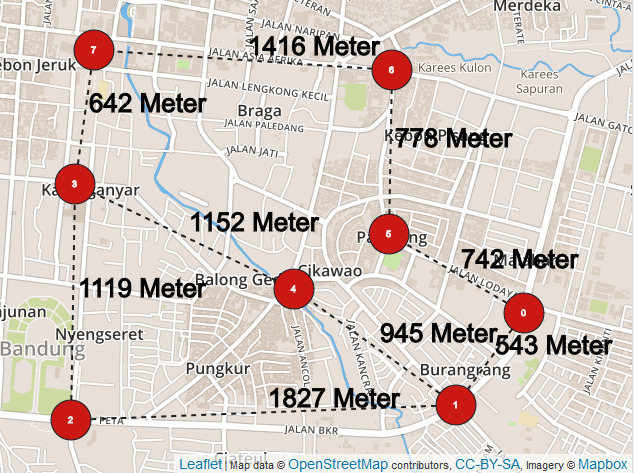
\includegraphics[scale=0.3]{figures/ALGORITMA/DATAMAP2.jpeg}
    \caption{Jalur Lokasi}
    \label{gambar22}
\end{figure}
    
\par Untuk jalur gambar \ref{gambar22} sudah terdapat bobot nilai yang tercantum yaitu jarak antara titik satu ke titik lainnya, bobot nilai ini akan di kumpulkan dan dibentuk kedalam table matriks agar dapat di proses pada tahap selanjutnya.
    
    
    
    

\section{Pemodelan Graf (Matriks Berbobot)}
\label{pemodelan_graf}
Pemodelan graf adalah graf yang setiap sisinya diberi sebuah bobot. Bobot pada tiap sisi dapat berbeda-beda bergantung pada masalah yang dimodelkan dengan graf. Bobot dapat menyatakan jarak antara dua buah kota atau titik, biaya perjalanan antara dua buah kota, waktu tempuh dari sebuah simpul ke simpul lain, ongkos produksi, dan sebagainya. Pemodelan graf dibentuk atas dasar sample data yang telah di kumpukan, dimana titik awal dan titik tujuan di hubungkan dengan bobot nilai tertentu kemudian membentuk sebuah jalur dalam bentuk graf. Secara umum sebelum dilakukan iterasi, algoritma sudah mengidenfikasi jarak terdekat dari node terdekatnya. Jika seluruh node berbobot tertentu yang (positif), maka node terdekat berikutnya dari node asal dapat ditemukan selama node berdekatan dengan node awal. Untuk graf yang dihasilkan dapat dilihat pada gambar \ref{gambar13}:

\begin{figure}[h]
    \centering
    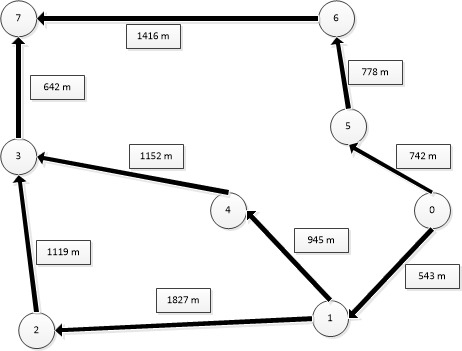
\includegraphics[scale=0.4]{figures/ALGORITMA/GRAF2.png}
    \caption{Graf Berbobot}
    \label{gambar13}
\end{figure}

\par Graf di atas dapat dilihat bahwa x adalah titik awal dan y adalah titik akhir. Graf di atas merupakan graf satu arah, hubungan graf diperoleh dari gambar \ref{gambar13}, dengan nilai jarak dan hubungan dari titik awal menuju titik akhir atau titik lainnya. Untuk matriks yang dihasilkan dari graf gambar \ref{gambar13}, dapat dilihat pada table matriks \ref{table13}:
\par Pada matriks dibawah merupakan gambaran dari graf berbobot dalam bentuk table matriks hubungan graf. Terdapat nilai yang diperoleh dari graf dan data dari hasil pengumpulan data lokasi dari google maps dan jarak yang diperoleh lalu dituliskan sesuai dengan data dari google maps dengan menghubungkan sumbu x sebagai awal dan sumbu y sebagai tujuan akhir jalur. Table matriks ini bernilai dengan satuan meter (m) dan untuk simbol "-" merupakan jarak yang tidak terjangkau atau tidak ada jalur terhadap titik tersebut.

\vspace{1cm}

\begin{table}[!htbp]
    \centering
    \caption{Matriks Hubungan Graf}
    \label{table13}
    \begin{tabular}{|l|l|l|l|l|l|l|l|l|}
    \hline
        & 0 & 1 & 2 & 3 & 4 & 5 & 6 & 7 \\
    \hline
        0 & 0 & 543 & - & - & - & 742 & - & - \\
    \hline
        1 & - & 0 & 1827 & - & 945 & - & - & - \\
    \hline
        2 & - & - & 0 & 1119 & - & - & - & - \\
    \hline
        3 & - & - & - & 0 & - & - & - & 647 \\
    \hline
        4 & - & - & - & 1152 & 0 & - & - & - \\
    \hline
        5 & - & - & - & - & - & 0 & 778 & - \\
    \hline
        6 & - & - & - & - & - & - & 0 & 1416 \\
    \hline
        7 & - & - & - & - & - & - & - & 0 \\
    \hline
    \end{tabular}
\end{table}


\chapter{ALGORITMA DIJKSTRA}
Algoritma Dijkstra (Jalur Terpendek Algoritma) adalah algoritma untuk menemukan jarak terpendek dari suatu vertex ke vertex yang lain pada suatu grafik yang berbobot, dimana jarak antar vertex adalah bobot dari setiap edge pada grafik tersebut \cite{salman2019minimum}.

\section{Algoritma Djikstra}
\label{Algoritma_Djikstra_Teori}
Algoritma Dijkstra dinamakan sesuai dengan nama penemunya, seorang ilmuwan komputer berkebangsaan Belanda yang bernama Edsger Dijkstra \cite{williams2019crusader}, adalah algoritma yang digunakan untuk mencari lintasan terpendek pada suatu graf berarah. Algoritma Dijkstra (Jalur Terpendek Algoritma) adalah algoritma untuk menemukan jarak terpendek dari suatu vertex ke vertex yang lain pada suatu grafik yang berbobot, dimana jarak antar vertex adalah bobot dari setiap edge pada grafik tersebut \cite{salman2019minimum}. Algoritma dijkstra mencari jarak terpendek untuk setiap titik dari suatu graph yang berbobot. Algoritma dijkstra mencari jarak terpendek dari simpul asal ke simpul terdekatnya, kemudian ke simpul kedua, dan seterusnya \cite{ghanbartehrani2019efficient}. Rumusa dalam algoritma ini adalah sebagai berikut:

\begin{equation}
\label{rumus_dijkstra_1}
    G = {V. E}
\end{equation}
\par Keterangan Rumus \ref{rumus_dijkstra_1}:
\par Sebuah grafik (G) didefenisikan oleh satu set simpul (Vertex = V) dan koleksi Edge (E).

Secara umum, sebelum dilakukan iterasi, vertex terdekatnya. Selama seluruh tepi berbobot tertentu yang (positif), maka vertex terdekat berikutnya dari node asal dapat ditemukan selama vertex bertemu dengan vertex Ti.
Kumpulan simpul yang lengkap dengan simpul di Ti dapat dianggap sebagai "simpul pinggiran". Vertex inilah yang merupakan kandidat dari algoritma dijkstra untuk memilih vertex berikutnya dari node asal. Algoritma Dijkstra merupakan salah satu varian bentuk algoritma populer dalam pemecahan persoalan yang terkait dengan masalah optimasi \cite{hellwig2019optimization}. Sifatnya sederhana dan lempang (straightforward) \cite{hidayat2019sistem}.

Ada beberapa kasus pencarian lintasan terpendek yang
diselesaikan menggunakan algoritma Dijkstra, yaitu:
\begin{enumerate}
    \item Pencarian lintasan terpendek antara dua buah simpul
tertentu (a pair shortest path),
    \item Pencarian lintasan terpendek antara semua pasangan
simpul (all pairs shortest path).
    \item Pencarian lintasan terpendek dari simpul tertentu ke
semua simpul yang lain (single-source shortest path).
    \item Pencarian lintasan terpendek antara dua buah simpul
yang melalui beberapa simpul tertentu (intermediate
shortest path)
\end{enumerate}

Algoritma ini bertujuan untuk menemukan jalur
terpendek berdasarkan bobot terkecil dari satu titik ke titik
lainnya. Misalkan titik mengambarkan gedung dan garis
menggambarkan jalan, maka algoritma Dijkstra melakukan
kalkulasi terhadap semua kemungkinan bobot terkecil dari
setiap titik.

\begin{figure}[h]
\centering
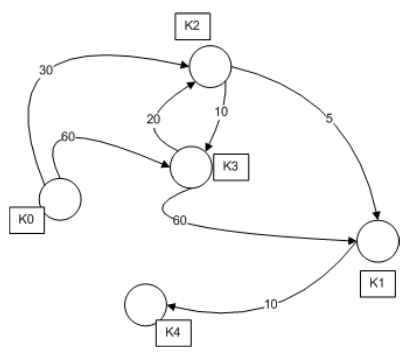
\includegraphics[scale=0.5]{figures/Algoritma_Dijkstra.PNG}
\caption{Algoritma Dijkstra}
\label{gambar2_9}
\end{figure}

Pertama-tama tentukan titik mana yang akan menjadi node awal, lalu beri bobot jarak pada node pertama ke node terdekat satu per satu, Dijkstra akan melakukan pengembangan pencarian dari satu titik ke titik lain dan ke itik selanjutnya tahap demi tahap. Inilah urutan logika dari lgoritma Dijkstra:
\begin{enumerate}
    \item Beri nilai bobot (jarak) untuk setiap titik ke titik
lainnya, lalu set nilai 0 pada node awal dan nilai tak
hingga terhadap node lain (belum terisi).
    \item Set semua node “Belum terjamah” dan set node awal
sebagai “Node keberangkatan”
    \item Dari node keberangkatan, pertimbangkan node
tetangga yang belum terjamah dan hitung jaraknya
dari titik keberangkatan. Sebagai contoh, jika titik keberangkatan K0 ke K2 memiliki bobot jarak 30 dan dari
K2 ke node K1 berjarak 5, maka jarak ke K1 melewati K2
menjadi 30+5=35. Jika jarak ini lebih kecil dari jarak
sebelumnya (yang telah terekam sebelumnya) hapus
data lama, simpan ulang data jarak dengan jarak yang
baru.
    \item Saat kita selesai mempertimbangkan setiap jarak
terhadap node tetangga, tandai node yang telah
terjamah sebagai “Node terjamah”. Node terjamah
tidak akan pernah di cek kembali, jarak yang disimpan
adalah jarak terakhir dan yang paling minimal
bobotnya.
    \item Set “Node belum terjamah” dengan jarak terkecil (dari
node keberangkatan) sebagai “Node Keberangkatan”
selanjutnya dan lanjutkan dengan kembali ke step 3.
\end{enumerate}

\section{Perhitungan Algoritma Djikstra}
\subsection{Analisis Algoritma Dijkstra}
Implementasi algoritma Dijkstra dilakukan untuk memperoleh rute terpendek yang bisa ditempuh dari suatu titik ke titik finish. Hasil yang diperoleh dari implementasi algoritma Dijkstra ini adalah rute terpendek yang terdiri dari node-node yang termasuk ke dalam solusi rute terpendek, dan total bobot minimumnya. Diskripsi matematis untuk grafik dapat diwakili G = \verb|{V. E}|, yang berarti sebuah grafik (G) didefenisikan oleh satu set simpul (Vertex = V) dan koleksi Edge (E).

Langkah-langkah algoritma Dijkstra dapat dilakukan dengan  langkah - langkah yang sudah di jelaskan pada poin \ref{Algoritma_Djikstra_Teori} bagian \ref{Algoritma_Djikstra_Teori} dan berikut tahap analisis yang dilakukan penulis dalam penerapan algoritma Dijkstra:

\begin{enumerate}
    \item Pada matriks hubungan graf table \ref{table51} sudah terdapat nilai dari setiap jalur yang akan dilewati, kemudian beri penamaan terhadap titik-titik lokasi tersebut dengan memberi label V sehingga seperti berikut :
    \par V(G)) = \verb|{V0, V1, V2, V3, V4, V5, V6, V7}|.
    
    \item Setelah titik-titik terbentuk, langkah selanjutnya adalah menghitung titik-titik yang saling berhubungan dengan cara berikut:
    \begin{enumerate}
        \item Dimulai dari menghitung G0 yaitu melihat node terdekat dari node0. Yang terdekat dari node0 adalah node1 dan node5. Node0 ke node1 memiliki jarak 543cm dan dari node0 ke node5 memiliki jarak 742cm. Nilai dari jumlah setiap jarak dimasukkan kedalam tabel V1 dan V5.

        \item Setelah itu menghitung G1 karena dari G0 nilai yang terkecil yaitu dari V1 dengan nilai 543, maka V1 terlebih dahulu yang dikerjakan atau yang dihitung jarak terhadap node yang terdekat dari V1. Selanjutnya menghitung jarak yang terhubung langsung dengan V1 yaitu V2 dan V4 dengan perhtiungan dihasilkan yaitu:
            \par G1 = V1 + (jumalah jarak node1 ke node2) = 2370
            \par G1 = V1 + (jumlah jarak node1 ke node4) = 1488
        
        \item Setelah itu menghitung G5 karena dari G1 nilai yang terkecil yaitu dari V5 dengan nilai 742, maka V5 terlebih dahulu yang dikerjakan atau yang dihitung jarak terhadap node yang terdekat dari V5. Selanjutnya menghitung jarak yang terhubung langsung dengan V5 yaitu V6 dengan perhtiungan dihasilkan yaitu:
            \par G5 = V5 + (jumalah jarak node5 ke node6) = 1520
            
        \item Setelah itu menghitung G4 karena dari G5 nilai yang terkecil yaitu dari V4 dengan nilai 1488, maka V4 terlebih dahulu yang dikerjakan atau yang dihitung jarak terhadap node yang terdekat dari V4. Selanjutnya menghitung jarak yang terhubung langsung dengan V4 yaitu V3 dengan perhtiungan dihasilkan yaitu:
            \par G4 = V4 + (jumalah jarak node4 ke node3) = 2640        

        \item Setelah itu menghitung G6 karena dari G4 nilai yang terkecil yaitu dari V6 dengan nilai 1520, maka V6 terlebih dahulu yang dikerjakan atau yang dihitung jarak terhadap node yang terdekat dari V6. Selanjutnya menghitung jarak yang terhubung langsung dengan V6 yaitu V3 dengan perhtiungan dihasilkan yaitu:
            \par G6 = V6 + (jumalah jarak node6 ke node7) = 2936

        \item Setelah itu menghitung G2 karena dari G6 nilai yang terkecil yaitu dari V2 dengan nilai 2370, maka V2 terlebih dahulu yang dikerjakan atau yang dihitung jarak terhadap node yang terdekat dari V2. Selanjutnya menghitung jarak yang terhubung langsung dengan V2 yaitu V3 dengan perhtiungan dihasilkan yaitu:
            \par G2 = V2 + (jumalah jarak node2 ke node3) = 3489
            \par Sebelumnya pada node3 sudah didapatkan jaraknya yaitu dari node 4 menuju node3 dengan nilai 2640, sedangkan nilai pada node2 menuju node3 adalah 3489. Jadi nilai yang tetap diambil adalah nilai terkceil yaitu 2640 nilai dari node4 menuju node3.

        \item Setelah itu menghitung G3 karena dari G2 nilai yang terkecil yaitu dari V3 dengan nilai 2640, maka V3 terlebih dahulu yang dikerjakan atau yang dihitung jarak terhadap node yang terdekat dari V3. Selanjutnya menghitung jarak yang terhubung langsung dengan V3 yaitu V7 dengan perhtiungan dihasilkan yaitu:
            \par G3 = V3 + (jumalah jarak node3 ke node7) = 3282
            \par Sebelumnya pada node7 sudah didapatkan jaraknya yaitu dari node 6 menuju node7 dengan nilai 2936, sedangkan nilai pada node3 menuju node7 adalah 3282. Jadi nilai yang tetap diambil adalah nilai terkceil yaitu 3282 nilai dari node6 menuju node7.
        
        \item Setelah itu G7 diturunkan saja.
        
        \item Dihasilkan table penyelesaian graf Dijkstra:
            \begin{figure}[h]
            \centering
            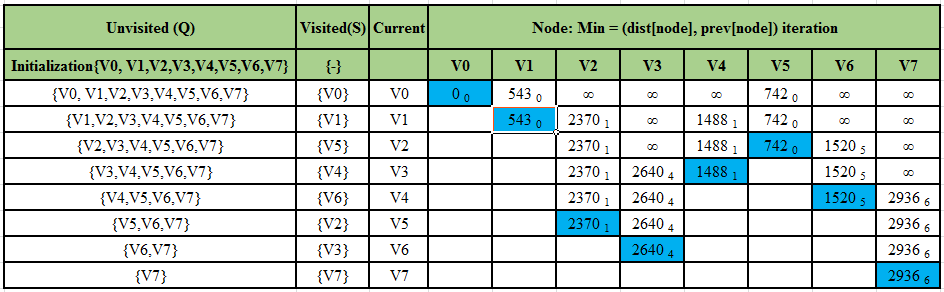
\includegraphics[scale=0.45]{figures/ALGORITMA/Matriks_Dijkstra.png}
            \caption{Matriks Dijkstra}
            \label{gambar52}
            \end{figure}
            
    \end{enumerate}
\end{enumerate}

Untuk membaca tabel perhitungan graf Dijkstra dan mengetahui lintasan mana yang terpendek yaitu:
\par 7 berasal dari node 6
\par 6 berasal dari node 5
\par 5 berasal dari node 0

Dari hasil yang didapatkan maka jalur yang terdekat yang diperoleh dari Algoritma Dijkstra adalah rute dengan titik V 0 \verb|->| 5 \verb|->| 6 \verb|->| 7 dengan jarak tempuh 2932 m. Adapun pseudocode yang akan diimplementasikan kedalam sistem berbasis web dari analisis algoritma Dijkstra adalah sebagai berikut :

\begin{lstlisting}[caption=Pseudocode Algoritma Dijkstra]
function Dijkstra(Graph, source):
      for each vertex v in Graph:                       
          dist[v] := infinity ;         
          previous[v] := undefined ;  
      end for                  
      
      dist[source] := 0 ;   
      Q := the set of all nodes in Graph ;        
      while Q is not empty:             
          u := vertex in Q with smallest distance in dist[] ;
          remove u from Q ;
          if dist[u] = infinity:
              break ;     
          end if        
          
          for each neighbor v of u:       
              alt := dist[u] + dist_between(u, v) ;
              if alt < dist[v]:  
                  dist[v] := alt ;
                  previous[v] := u ;
                  decrease-key v in Q;    
              end if
          end for
          
      end while
      
  return dist;
\end{lstlisting}
\label{PseudocodeAlgoritmaDijkstra}

\chapter{ALGORITMA FLOYD WARSHALL}
Algoritma Floyd-Warshall adalah salah satu varian dari pemrograman dinamis, yaitu suatu metode yang melakukan pemecahan dengan memandang solusi yang akan diperoleh sebagai suatu keputusan yang saling terkait. Artinya solusi-solusi tersebut dibentuk dari solusi yang berasal dari tahap sebelumnya dan ada kemungkinan solusi lebih dari satu Algoritma Floyd Warshall adalah dengan membandingkan semua lintasan yang mungkin terjadi dalam graf untuk setiap pasang simpul dan melakukan pengujian dari setiap kombinasi simpul yang diperoleh \cite{novianti2019implementasi}.

\section{Algoritma Floyd Warshall}
Algoritma Floyd-Warshall adalah salah satu varian dari pemrograman dinamis, yaitu suatu metode yang melakukan pemecahan dengan memandang solusi yang akan diperoleh sebagai suatu keputusan yang saling terkait. Artinya solusi-solusi tersebut dibentuk dari solusi yang berasal dari tahap sebelumnya dan ada kemungkinan solusi lebih dari satu Algoritma Floyd Warshall adalah dengan membandingkan semua lintasan yang mungkin terjadi dalam graf untuk setiap pasang simpul dan melakukan pengujian dari setiap kombinasi simpul yang diperoleh \cite{novianti2019implementasi}.
Algoritma Floyd Warshall ditemukan oleh Warshall untuk mencari path terpendek merupakan algoritma yang sederhana dan mudah implementasikannya. Algoritma Floyd Warshall adalah matriks hubung graf berarah berlabel, dan keluarannya adalah path terpendek dari semua titik kesemua titik. Dalam usaha mencari jalur terpendek, algoritma Warshall memulai iterasi dari titik awalnya kemudian memperpanjang path dengan mengevaluasi titik demi titik hingga mencapai titik tujuan dengan jumlah bobot yang seminimum mungkin \cite{hasibuan2016penerapan}.
mekanisme dari algoritma FloydWarshall ini terdiri dari beberapa langkah yang harus dilakukan, yaitu \cite{darnita2017implementasi}:
\begin{enumerate}
    \item Langkah awal yang harus dilakukan untuk menentukan shortest path dengan menggunakan algoritma Floyd-Warshall adalah dengan merepresentasikan suatu graf sebagai suatu matriks berbobot.
    \item Langkah kedua adalah melakukan dekomposisi.
    \item Langkah ketiga adalah menentukan struktur shortest path. Dalam hal ini, harus dilakukan dua pengamatan terlebih dahulu sebelum melangkah lebih jauh.
    \item Dilakukan penentuan shortest path
    \item Melakukan iterasi yang dimulai dari iterasi ke 0 sampai dengan.
\end{enumerate}

Hasil akhir dari algoritma Floyd-Warshall adalah matriks untuk iterasi ke-n. Dari matriks ken ini, dapat dilihat shortest path untuk setiap vertex pada suatu graph.

Misalkan terdapat suatu graf G dengan simpul-simpul V yang  masing-masing  bernomor  1  s.d.  N  (sebanyak  N  buah).      Misalkan      pula      terdapat      suatu      fungsi      shortestPath(i,   j,   k)    yang    mengembalikan    kemungkinan  jalur  terpendek  dari  i  ke  j  dengan  hanya  memanfaatkan simpul 1 s.d. k sebagai titik perantara. Tujuan   akhir   penggunaan   fungsi   ini   adalah   untuk   mencari  jalur  terpendek  dari  setiap  simpul  i  ke  simpul  j  dengan perantara simpul 1 s.d. k+1. 

Ada dua kemungkinan yang terjadi:  
\begin{enumerate}
    \item Jalur terpendek yang sebenarnya hanya berasal dari simpul-simpul yang berada antara 1 hingga k. 
    \item Ada sebagian jalur yang berasal dari simpul-simpul i s.d. k+1, dan juga dari k+1 hingga j.
\end{enumerate}{}

Perlu  diketahui  bahwa  jalur  terpendek  dari  i  ke  j  yang  hanya  melewati  simpul  1  s.d.  k  telah  didefinisikan  pada  fungsi  shortestPath(i,  j,  k)  dan  telah  jelas  bahwa  jika  ada  solusi  dari  i  s.d.  k+1  hingga  j,  maka  panjang  dari  solusi  tadi adalah jumlah (konkatenasi) dari jalur terpendek dari i s.d. k+1 (yang melewati simpul-simpul 1 s.d. k), dan jalur terpendek  dari  k+1  s.d.  j  (juga  menggunakan  simpul-simpul dari 1 s.d. k).

Maka  dari  itu,  rumus  untuk  fungsi  shortestPath(i, j, k) bisa ditulis sebagai:
\begin{equation}
    \label{label21}
    X[i,j] ≤ X[i,k] + X[k,j]
\end{equation}
    \par Keterangan \ref{label21}:
        \par X = Matriks
        \par i = titik awal
        \par j = titik akhir
        \par k = iterasi 1 sampai ke n

Algoritma ini bertujuan untuk menemukan jalur
terpendek berdasarkan bobot terkecil dari satu titik ke titik
lainnya. Misalkan titik mengambarkan gedung dan garis
menggambarkan jalan, maka algoritma Dijkstra melakukan
kalkulasi terhadap semua kemungkinan bobot terkecil dari
setiap titik.

\section{Perhitungan Algoritma Floyd Warshall}
\subsection{Analisis Algoritma Floyd Warshall}
Algoritma Floyd Warshall sangat efisien dari sudut pandang penyimpanan data kare-na dapat diimplementasikan dengan hanya pengubahan sebuah matriks jarak. Adapun mekanisme dari algoritma Floyd-Warshall ini terdiri dari beberapa langkah yang harus dilakukan, yaitu:

\begin{enumerate}
    \item Langkah awal yang harus dilakukan untuk menentukan shortest path dengan menggunakan algoritma Floyd Warshall adalah dengan merepresentasikan suatu graf sebagai suatu matriks berbobot (dapat dilihat pada bagian \ref{pemodelan_graf}).
    \item Langkah kedua adalah melakukan dekomposisi Floyd-Warshall atau membentuk sebuah table matriks dan titik yang akan dihitung (dapat dilihat pada bagian \ref{pemodelan_graf}).
    
    \begin{enumerate}
        \item Hasil yang didapatkan dari graf adalah
            \begin{verbatim}
                K	=	0, 1, 2, 3, 4, 5, 6, 7
                i	=	0, 1, 2, 3, 4, 5, 6, 7
                j	=	0, 1, 2, 3, 4, 5, 6, 7
            \end{verbatim}
        
        \item Untuk rumus yang digunakan:
            \begin{equation}
                Rumus X[i,j] < X[i,k] + X[k,j]
            \end{equation}
            \par Penjelasan lebih dapat dilihat pada point \ref{label21}.
        
        \item Untuk table matriks hubungan graf, terdapat tujuh table Matriks hubungan graf, dimana setiap table meilihki proses yang sama namun dengan nilai matriks yang berubah-ubah. Adapun table matriks yang dihasilkan diberi penamaan dengan table matriks hubungan graf.
        
        \item Langkah selanjutnya, menentukan struktur shortest path kemudian melaku-kan penentuan shortest path dari i ke j yang memuat vertex k.


    \begin{enumerate}
    \item Matriks hubungan graf, K=0:            \begin{table}[!htbp]
    \centering
    \caption{Matriks hubungan graf, K=0}
    \label{table52}
    \begin{tabular}{|l|l|l|l|l|l|l|l|l|}                \hline
         X0 & V0 & V1 & V2 & V3 & V4 & V5 & V6 & V7 \\
    \hline
         V0 & 0 & 543 & - & - & - & 742 & - & - \\
    \hline
          V1 & - & 0 & 1827 & - & 945 & - & - & - \\
    \hline
         V2 & - & - & 0 & 1119 & - & - & - & - \\
    \hline
         V3 & - & - & - & 0 & - & - & - & 647 \\
    \hline
         V4 & - & - & - & 1152 & 0 & - & - & - \\
    \hline
        V5 & - & - & - & - & - & 0 & 778 & - \\
    \hline
        V6 & - & - & - & - & - & 0 & 28.93 & - \\
    \hline
        V7 & - & - & - & - & - & 0 & - & - \\
    \hline
    \end{tabular}
    \end{table}


            \par Penyelesaian:
            \begin{figure}[h]
            \centering
            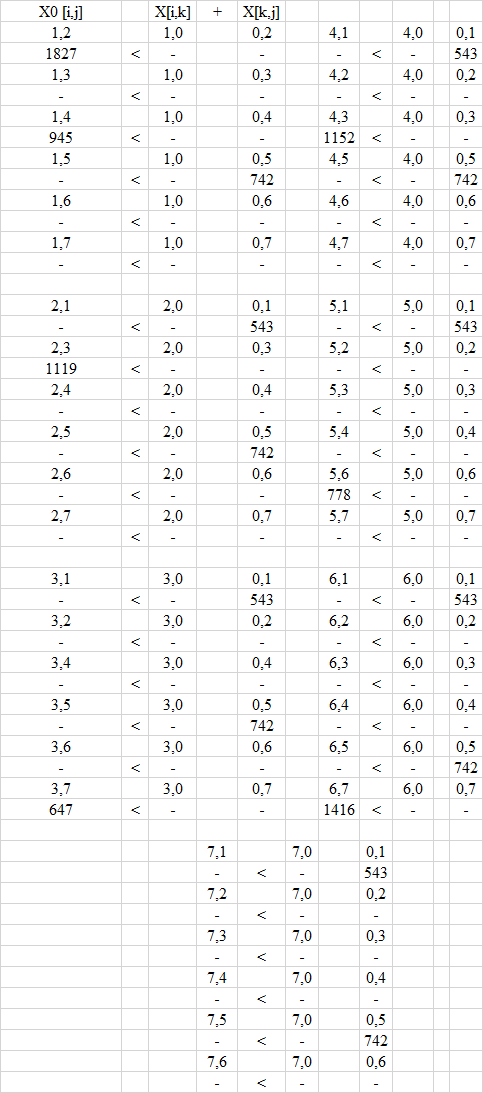
\includegraphics[scale=0.34]{figures/ALGORITMA/MATRIKSX0.png}
            \caption{Matriks X0}
            \label{gambar31}
            \end{figure}
            \par Untuk iterasi terhadap matriks K=0 tidak terdapat jalur dan setiap sel matriks W dicek apakah \verb|X[i,j] < X[i,k] + X[k,j]| jika ya maka \verb|X[i,j]| digannti dengan \verb|X[i,k] + X[k,j]|


            \item Matriks hubungan graf, K=1:
                \begin{table}[!htbp]
                \centering
                \caption{Matriks hubungan graf, K=1}
                \label{table32}
                    \begin{tabular}{|l|l|l|l|l|l|l|l|l|}
                    \hline
                        X1 & V0 & V1 & V2 & V3 & V4 & V5 & V6 & V7 \\
                    \hline
                        V0 & 0 & 543 & 2370 & - & 1488 & 742 & - & - \\
                    \hline
                        V1 & - & 0 & 1827 & - & 945 & - & - & - \\
                    \hline
                        V2 & - & - & 0 & 1119 & - & - & - & - \\
                    \hline
                        V3 & - & - & - & 0 & - & - & - & 647 \\
                    \hline
                        V4 & - & - & - & 1152 & 0 & - & - & - \\
                    \hline
                        V5 & - & - & - & - & - & 0 & 778 & - \\
                    \hline
                       V6 & - & - & - & - & - & 0 & 28.93 & - \\
                    \hline
                       V7 & - & - & - & - & - & 0 & - & - \\
                    \hline
                \end{tabular}
                \end{table}
            \par Penyelesaian:
\begin{verbatim}
X1 [i,j] > X[i,k]	+	X[k,j]
0,2	> 0,1	+	1,2
-	> 543	+	1827

0,4	> 0,1 +	1,4
- > 543	+ 945
\end{verbatim}

            \par Karena \verb|X1[0,2]| lebih besar dari jumlah \verb|X[0,1] + X[1,2]|, maka nilai \verb|X1[0,2]| diubah menjadi nilai total \verb|X[0,1] + X[1,2]| yaitu 2370 m. Dan \verb|X1[0,4]| lebih besar dari jumlah \verb|X[0,1] + X[1,4]|, maka nilai \verb|X1[0,4]| diubah menjadi nilai total \verb|X[0,1] + X[1,4]| yaitu 1488 m. Ini menandakan bahwa pada X1, terdapat rute untuk menuju node ke 2 dan 4. jalur yang terbentuk adalah 0 \verb|->| 1 \verb|->| 2 dan 0 \verb|->| 1 \verb|->| 4.
            
            \vspace{6.5cm}
            
            \item  Matriks hubungan graf, K=2:
                \begin{table}[!htbp]
                \centering
                \caption{Matriks hubungan graf, K=2}
                \label{table33}
                    \begin{tabular}{|l|l|l|l|l|l|l|l|l|}
                    \hline
                        X2 & V0 & V1 & V2 & V3 & V4 & V5 & V6 & V7 \\
                    \hline
                        V0 & 0 & 543 & 2370 & 3489 & 1488 & 742 & - & - \\
                    \hline
                        V1 & - & 0 & 1827 & 2946 & 945 & - & - & - \\
                    \hline
                        V2 & - & - & 0 & 1119 & - & - & - & - \\
                    \hline
                        V3 & - & - & - & 0 & - & - & - & 647 \\
                    \hline
                        V4 & - & - & - & 1152 & 0 & - & - & - \\
                    \hline
                        V5 & - & - & - & - & - & 0 & 778 & - \\
                    \hline
                       V6 & - & - & - & - & - & 0 & 28.93 & - \\
                    \hline
                       V7 & - & - & - & - & - & 0 & - & - \\
                    \hline
                \end{tabular}
                \end{table}
            \par Penyelesaian:
\begin{verbatim}
X2[i,j] > X[i,k] + X[k,j]
0,3 > 0,2 + 2,3
- > 2370 + 1119

1,3 > 1,2 + 2,3
- > 1827 + 1119
\end{verbatim}

            \par Karena \verb|X2[0,3]| lebih besar dari jumlah \verb|X[0,2] + X[2,3]|, maka nilai \verb|X2[1,3]| diubah menjadi nilai total \verb|X[1,2] + X[2,3]|. Sehingga jalur yang dihasilkan pada matriks graf K=2 adalah 0 \verb|->| 2 \verb|->| 3 dan 1 \verb|->| 2 \verb|->| 3.
            
            \vspace{0.3cm}
            
            \item  Matriks hubungan graf, K=3:
                \begin{table}[!htbp]
                \centering
                \caption{Matriks hubungan graf, K=3}
                \label{table34}
                    \begin{tabular}{|l|l|l|l|l|l|l|l|l|}
                    \hline
                        X3 & V0 & V1 & V2 & V3 & V4 & V5 & V6 & V7 \\
                    \hline
                        V0 & 0 & 543 & 2370 & 3489 & 1488 & 742 & - & 4136 \\
                    \hline
                        V1 & - & 0 & 1827 & 2946 & 945 & - & - & 3593 \\
                    \hline
                        V2 & - & - & 0 & 1119 & - & - & - & 1766 \\
                    \hline
                        V3 & - & - & - & 0 & - & - & - & 647 \\
                    \hline
                        V4 & - & - & - & 1152 & 0 & - & - & 1799 \\
                    \hline
                        V5 & - & - & - & - & - & 0 & 778 & - \\
                    \hline
                       V6 & - & - & - & - & - & 0 & 28.93 & - \\
                    \hline
                       V7 & - & - & - & - & - & 0 & - & - \\
                    \hline
                \end{tabular}
                \end{table}
                
                \vspace{1cm}
                
            \par Penyelesaian:
\begin{verbatim}
X3[i,j] > X[i,k] + X[k,j]
0,7 > 0,3 + 3,7
- > 3489 + 647

1,7 > 1,3 + 3,7
- > 2946 + 647

2,7 > 2,3 + 3,7
- > 1119 + 647

4,7 > 4,3 + 3,7
- > 1152 + 647
\end{verbatim}
            \par Karena \verb|X3[0,7]| lebih besar dari jumlah \verb|X[0,3] + X[3,7]|, maka nilai \verb|X2[0,7]| diubah menjadi nilai total \verb|X[0,3] + X[3,7]|. Sehingga jalur yang dihasilkan pada matriks graf K=3 adalah 0 \verb|->| 3 \verb|->| 7. Dan untuk nilai x[1,7], x[2,7], x[4,7] juga diubah.

\vspace{0.3cm}

            \item  Matriks hubungan graf, K=4:
            \par Penyelesaian:
\begin{verbatim}
X4[i,j] > X[i,k] + X[k,j]
0,7 > 0,4 + 4,7
4136 > 1488 + 1799

1,3 > 1,4 + 4,3
2946 > 945 + 1152

1,7 > 1,4 + 4,7
3593 > 945 + 1799
\end{verbatim}
            \par Karena \verb|X3[0,7]| lebih besar dari jumlah \verb|X[0,4] + X[4,7]|, maka nilai \verb|X3[0,7]| diubah menjadi nilai total \verb|X[0,4] + X[4,7]|. Sehingga jalur yang dihasilkan pada matriks graf K=3 adalah 0 \verb|->| 4 \verb|->| 7. Dan untuk nilai x[1,3], x[1,7]juga diubah. Untuk matriks selanjutnya juga di hitung dengan car yang sama sehinnga dihasilkan beberapa titik jalur dan perubahan matriks pada setiap matriks K. Kemudian pada Matriks hubungan graf, K=5,K=6 dan K=7 tidak terjadi perubahan pada matriksnya.
        \end{enumerate}
    \end{enumerate}
    
    
    
    \item Setelah melakukan perhitungan table matriks graf, langkah selanjutnya kemudian melakukan iterasi yang dimulai dari iterasi ke 0 sampai dengan n. Adapun hasil akhir table matriks hubungan graf K sebagai berikut:
    
    \vspace{1.5cm}
    
        \begin{table}[!htbp]
        \centering
        \caption{Hasil Akhir Matriks hubungan graf, K}
        \label{table35}
            \begin{tabular}{|l|l|l|l|l|l|l|l|l|}
            \hline
                Dari/Ke & 0 & 1 & 2 & 3 & 4 & 5 & 6 & 7 \\
            \hline
                0 & 0 & 543 & 2370 & 3489 & 1488 & 742 & - & 3287 \\
            \hline
                1 & - & 0 & 1827 & 2097 & 945 & - & - & 2744 \\
            \hline
                2 & - & - & 0 & 1119 & - & - & - & 1766 \\
            \hline
                3 & - & - & - & 0 & - & - & - & 647 \\
            \hline
                4 & - & - & - & 1152 & 0 & - & - & 1799 \\
            \hline
                5 & - & - & - & - & - & 0 & 778 & - \\
            \hline
                6 & - & - & - & - & - & - & 0 & 1416 \\
            \hline
                7 & - & - & - & - & - & - & - & 0 \\
            \hline
        \end{tabular}
        \end{table}
        
    \par Kemudian dihasilkan jalur dari peritungan tersebut:
\begin{verbatim}
0 -> 5 -> 6 -> 7 Dengan Jarak 2936 m
0 -> 1 -> 2 -> 3 -> 7 Dengan Jarak 4136 m
0 -> 1 -> 4 -> 3 -> 7 Dengan Jarak 3287 m
\end{verbatim}
        
        \item Hasil akhir dari algoritma ini adalah jalur tependek yang dihasilkan dari iterasi matriks graf, sehingga dihasilkan jalur dengan node 0 \verb|->| 5 \verb|->| 6 \verb|->| 7 dengan jarak 2936 m. Adapun pseudocode yang akan diimplementasikan kedalam sistem berbasis web dari analisis algoritma Floyd Warshall adalah sebagai berikut:
        
\begin{lstlisting}[caption=Pseudocode Algoritma Floyd Warshall]
    function floydwarshall(int[1..n,1..n] graph) {
        // Inisialisasi
        var int[1..n,1..n] jarak:= graph
        var int[1..n,1..n] sebelum
        for i from 1 to n
            for j from 1 to n
                if jarak[i,j] < Tak-hingga
                    sebelum[i,j]:= i
        // Perulangan utama pada algoritme
        for k from 1 to n
            for i from 1 to n
                for j from 1 to n
                    if jarak[i,j] > jarak[i,k] + jarak[k,j]
                        jarak[i,j] = jarak[i,k] + jarak[k,j]
                        sebelum[i,j] = sebelum[k,j]
        return jarak
    }
\end{lstlisting}
\label{PseudocodeAlgoritmaFloydWarshall}
\end{enumerate}

\chapter{PERBANDINGAN ALGORITMA}
Pengujian ini dilakukan secara bergantian menggunakan algoritma Dijkstra dan Algoritma Floyd Warshall dengan titik yang sama kemudian dilakukan perbandingan dengan kedua algoritma.

\section{PERBANDINGAN ALGORITMA DIJKSTRA DAN FLOYD WARSHALL}
Menghitung jalur terpendek dengan mencari jarak antara jalur-jalur yang ada. Menentukan rute optimal dengan parameter waktu tempuh tercepat setelah melakukan pengolahan data dengan menggunakan algoritma Dijkstra dan algoritma Floyd-Warshall. Dari perbandingan kedua algoritma tersebut memiliki tingkat akurasi hasil yang sama. Namun kedua algoritma ini memiliki cara dan fungsi berbeda untuk mencari rute terdekat dan hasil yang diperoleh kedua algoritma tersebut memiliki jalur yang sama. Hasil setiap masing-masing algoritma yang telah di analisis maka dihasilkan berikut table perbandingan dengan kedua algoritma:
\vspace{4cm}
    \begin{table}[!htbp]
    \centering
    \caption{Perbandingan Algoritma Dijsktra Dan Floyd-Warshall}
    \label{table31}
        \begin{tabular}{|l|l|l|l|}
        \hline
            & Algoritma Dijkstra & Algoritma Floyd Warshall & Akurasi \\
        \hline
            Rute &  0 \verb|->| 5 \verb|->| 6 \verb|->| 7 &  0 \verb|->| 5 \verb|->| 6 \verb|->| 7 & Sama \\
        \hline
            Jarak & 2936 m & 2936 m & Sama \\
        \hline
            Matriks & Matriks Dijsktra & Matriks Graf K & Beda \\
        \hline
    \end{tabular}
    \end{table}
    
    

\chapter{XAMPP (PHP VERSI 7)}
Xampp adalah perangkat lunak bebas, yang mendukung banyak sistem operasi, merupakan kompilasi dari beberapa program,  Fungsinya adalah sebagai server yang berdiri sendiri (localhost) \cite{siregar2018rancang}. Xampp merupakan singkatan dari X (empat sistem operasi apapun), Apache, Mysql, PHP, dan Perl. Xampp adalah tool yang menyediakan paket perangkat lunak dalam satu buah paket. Dalam paket Xampp sudah terdapat Apache (web server), Mysql (database), PHP (server side scripting), Perl ,FTP server, PhpMyAdmin dan berbagai pustaka bantu lainya. XAMPP adalah perangkat lunak bebas, yang mendukung banyak sistem operasi, merupakan kompilasi dari beberapa program \cite{sugiarto2019aplikasi}.

Dari definisi tersebut, penulis menyimpulkan bahwa XAMPP adalah sebuah software yang berfungsi untuk menjalankan website berbasis PHP dan menggunakan pengolah data MySQL di komputer lokal. XAMPP berperan sebagai server web pada komputer. XAMPP juga dapat disebut sebuah cpanel server virtual, yang dapat membantu melakukan preview sehingga dapat memodifikasi website tanpa harus online atau terakses dengan internet.

Program ini tersedia dalam GNU General Public License dan bebas,
merupakan web server yang mudah digunakan yang dapat melayani tampilan
halaman web yang dinamis. Selain itu XAMMP adalah 100\verb|%| open source, tersedia bebas dan legal \cite{siregar2017perancangan}.

\section{Tutorial Install Xampp}
\begin{enumerate}
    \item Download terlebih dahulu aplikasi Xampp di \textbf{\textit{https://www.apachefriends.org/ index.html}}, download sesuai sistem operasi yang anda gunakan, pada tutorial kali ini saya akan melakukan instalasi XAMPP di Windows 10.
    
	\item Setelah download aplikasi, lakukan instalasi XAMPP, dengan cara klik kanan pada file instalasi kemudian pilih Open.
		\begin{figure}[!htbp]
    		\centering
    		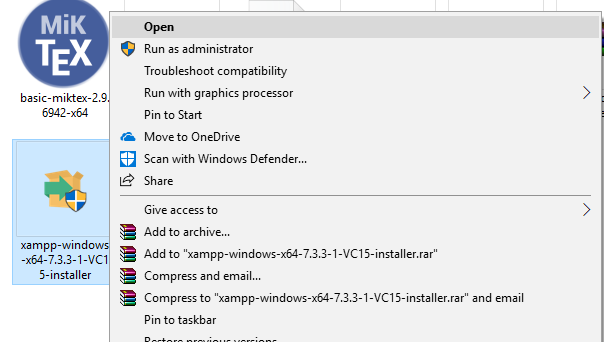
\includegraphics[width=0.7\textwidth]{figures/XAMPP/Xampp2.png}
    		\label{Xampp2}
		\end{figure}
		
	\item Jika pada saat melakukan instalasi muncul peringatan yang bertujuan untuk memastikan apakah Anda akan menginstal aplikasi ini, Silakan klik Ok/Yes untuk melanjutkan instalasi.
		\begin{figure}[!htbp]
    		\centering
    		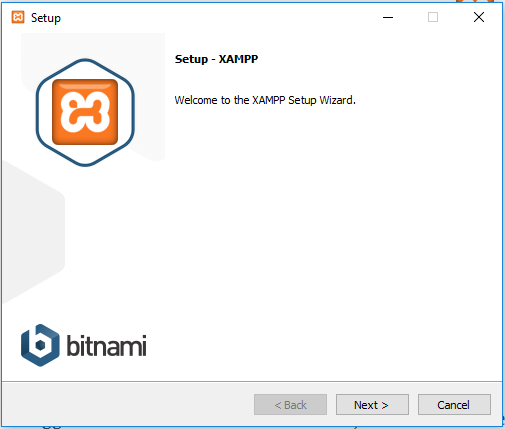
\includegraphics[width=0.7\textwidth]{figures/XAMPP/Xampp3.PNG}
    		\label{Xampp3}
		\end{figure}
		
	\item Klik next untuk melanjutkan, kemudian akan tampil pilihan aplikasi apa yang akan Anda install dan tidak ingin Anda install.
		\begin{figure}[!htbp]
    		\centering
    		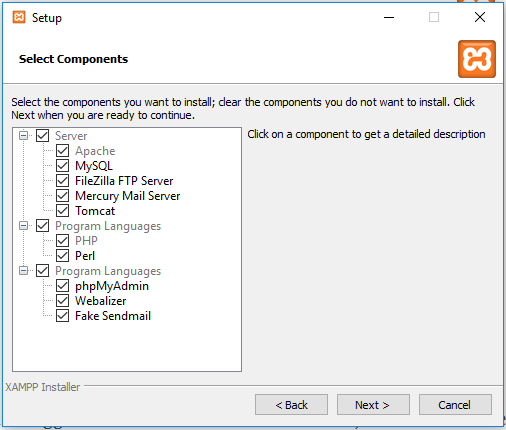
\includegraphics[width=0.5\textwidth]{figures/XAMPP/Xampp4.PNG}
    		\label{Xampp4}
		\end{figure}
		
	\item Tahap selanjutnya adalah memilih folder dimana lokasi instalasi xampp akan disimpan.
		\begin{figure}[!htbp]
    		\centering
    		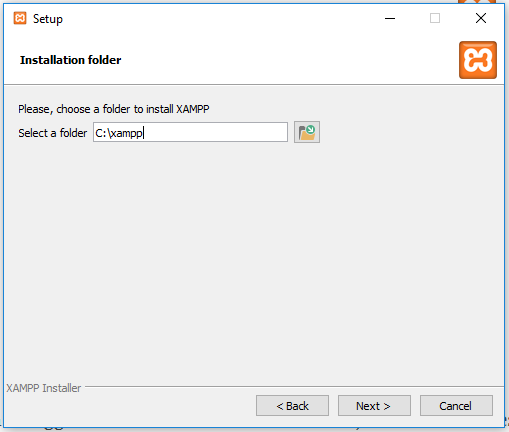
\includegraphics[width=0.5\textwidth]{figures/XAMPP/Xampp5.PNG}
    		\label{Xampp5}
		\end{figure}
		
	\item Silakan hilangkan centang pada “Learn more about Bitnami for XAMPP”, kemudian klik Next.
		\begin{figure}[!htbp]
    		\centering
    		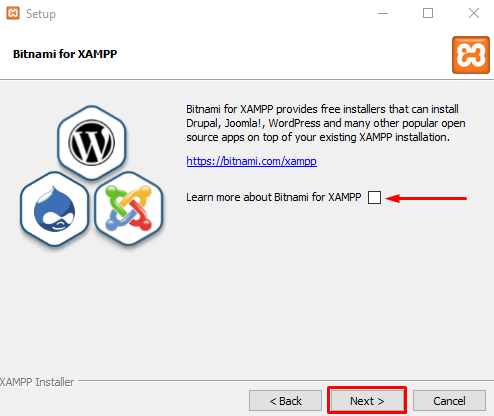
\includegraphics[width=0.5\textwidth]{figures/XAMPP/Xampp6.png}
    		\label{Xampp6}
		\end{figure}
		
	\item Klik next untuk malnjutkan ke proses instalasi xampp.
		\begin{figure}[!htbp]
    		\centering
    		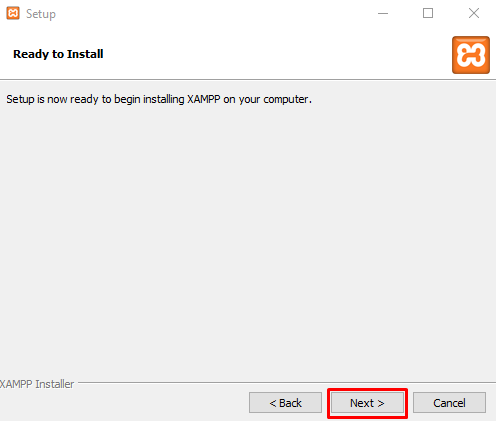
\includegraphics[width=0.7\textwidth]{figures/XAMPP/Xampp7.png}
    		\label{Xampp7}
		\end{figure}
		
	\item Apabila aplikasi sudah terinstal maka akan tampil pertanyaan mengenai apakah Anda ingin langsung menjalankan control panel. Pastikan pilihan tersebut sudah tercentang, kemudian klik tombol Finish.
		\begin{figure}[!htbp]
    		\centering
    		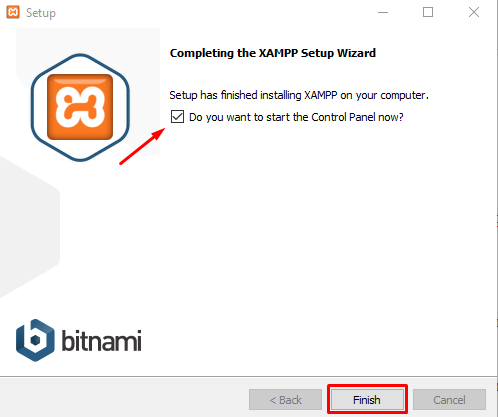
\includegraphics[width=0.8\textwidth]{figures/XAMPP/Xampp8.png}
    		\label{Xampp8}
		\end{figure}
		
	\item Control panel akan muncul otomatis, tapi jika Anda tidak mencentang pilihan di halaman sebelumnya, maka Anda perlu membuka langsung control panel melalui start menu atau folder XAMPP di komputer Anda.
	
	\item Apabila control panel sudah muncul dan terlihat seperti gambar \ref{Xampp9}, maka proses instalasi Xampp berhasil.
		\begin{figure}[!htbp]
    		\centering
    		\caption{Control Panel Xampp}
    		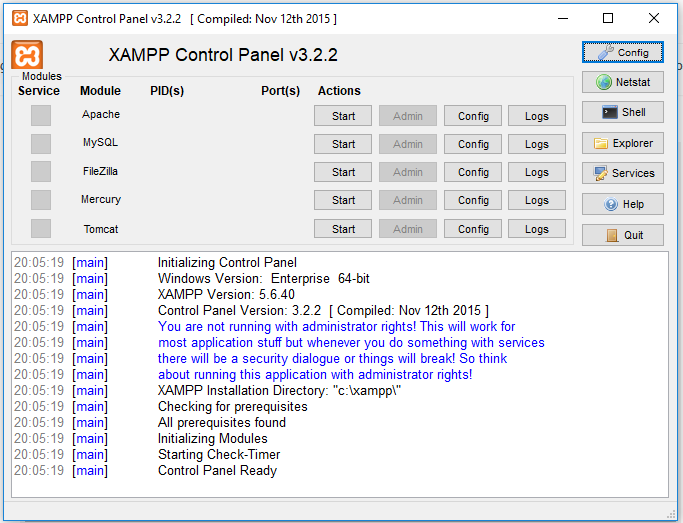
\includegraphics[width=0.8\textwidth]{figures/XAMPP/Xampp9.PNG}
    		\label{Xampp9}
		\end{figure}
\end{enumerate}

\section{Mengatasi Error Pada Xampp}
Hal yang menjadi penyebab utama kenapa tampil error pada XAMPP biasanya disebabkan aplikasi lain pada komputer Anda menggunakan port 80 atau 443, dimana port tersebut digunakan oleh Apache dan MySQL. Berikut cara mengatasi error pada xampp:
\begin{enumerate}
    \item Klik Start, kemudian ketikkan “services.msc” pilih Services yang ada di bagian Best match.
    \item Scrol ke bawah, pada bagian World Wide Web Publishing Service klik kanan dan pilih Stop.
    \item Silakan close XAMPP, kemudian buka kembali dan jalankan Apache dan MySQL pada XAMPP.
\end{enumerate}

Jika langkah yang Anda lakukan tidak berhasil mengatasi masalah yang dihadapi atau tidak menemukan World Wide Web Publishing, silakan lakukan langkah di bawah ini:
\begin{enumerate}
    \item Buka control panel melalui tombol start yang ada pada pojok kiri bawah
    
    \item Kemudian pilih system and security
		\begin{figure}[!htbp]
    		\centering
    		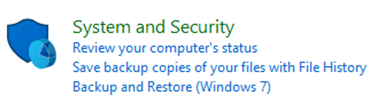
\includegraphics[width=0.5\textwidth]{figures/XAMPP/Xampp12.PNG}
    		\label{Xampp12}
		\end{figure}
		
	\item Pilih windows defender firewall
		\begin{figure}[!htbp]
    		\centering
    		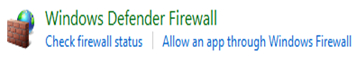
\includegraphics[width=0.5\textwidth]{figures/XAMPP/Xampp13.PNG}
    		\label{Xampp13}
		\end{figure}
		
	\item Pilih advanced settings
		\begin{figure}[!htbp]
    		\centering
    		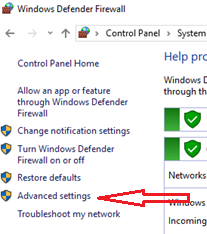
\includegraphics[width=0.5\textwidth]{figures/XAMPP/Xampp14.PNG}
    		\label{Xampp14}
		\end{figure}
		
	\item Klik Inbound dan klik kanan kemudian pilih New Rule, dapat dilihat seperti pada gambar dibawah
		\begin{figure}[!htbp]
    		\centering
    		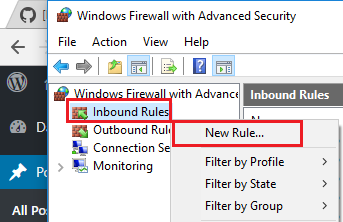
\includegraphics[width=0.4\textwidth]{figures/XAMPP/Xampp15.png}
    		\label{Xampp15}
		\end{figure}
		
	\item Pilih Port dan tekan tombol Next, kemudian pada kolom Specific Ports isi dengan 80, 443 kemudian klik Next.
		\begin{figure}[!htbp]
    		\centering
    		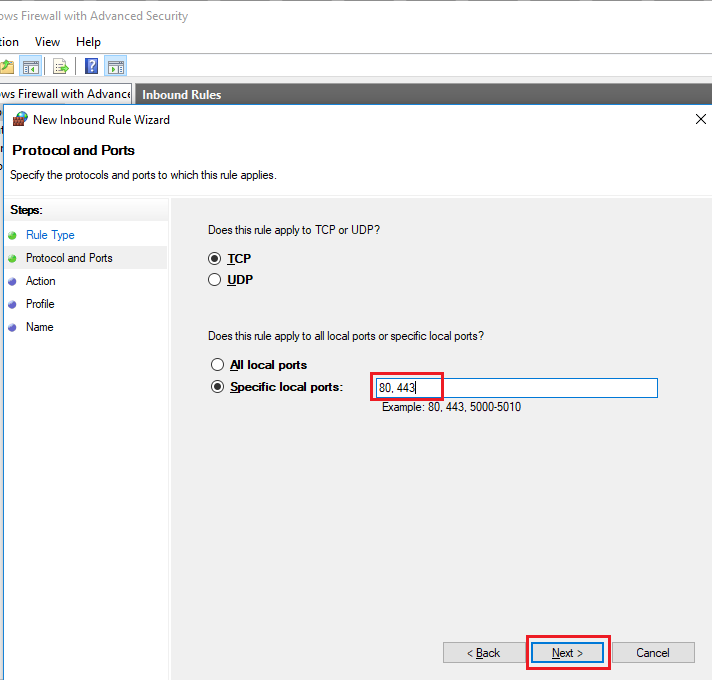
\includegraphics[width=0.7\textwidth]{figures/XAMPP/Xampp16.png}
    		\label{Xampp16}
		\end{figure}
		
	\item Centang Allow the Connection kemudian klik Next
		\begin{figure}[!htbp]
    		\centering
    		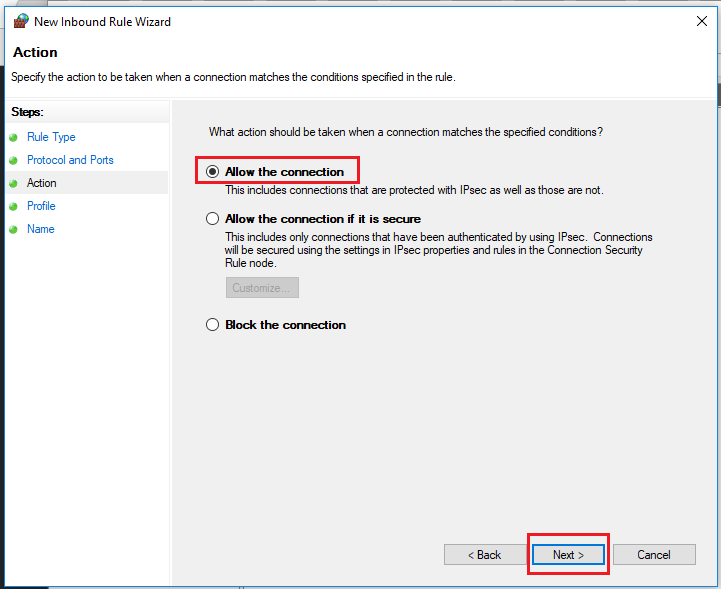
\includegraphics[width=0.7\textwidth]{figures/XAMPP/Xampp17.png}
    		\label{Xampp17}
		\end{figure}
		
	\item Pastikan semua pilihan dicentang seperti pada gambar dibawah, kemudian klik Next
		\begin{figure}[!htbp]
    		\centering
    		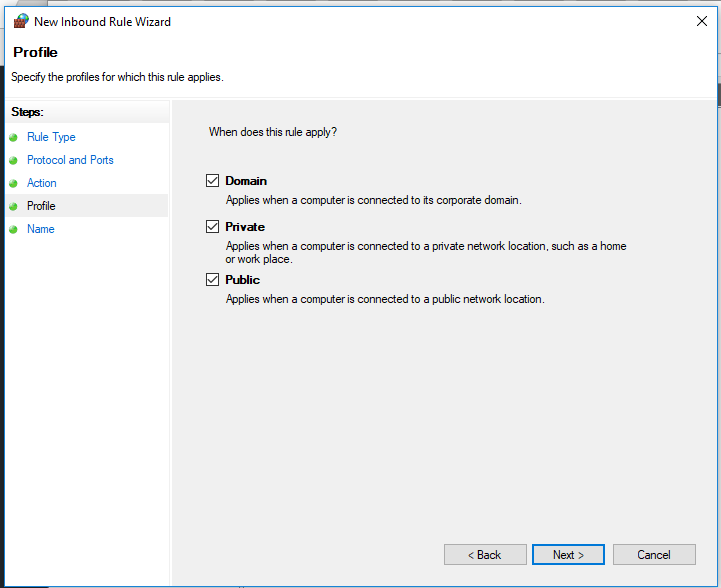
\includegraphics[width=0.7\textwidth]{figures/XAMPP/Xampp18.png}
    		\label{Xampp18}
		\end{figure}
		
	\item Masukkan lokal1 pada kolom name, kemudian klik Finish
		\begin{figure}[!htbp]
    		\centering
    		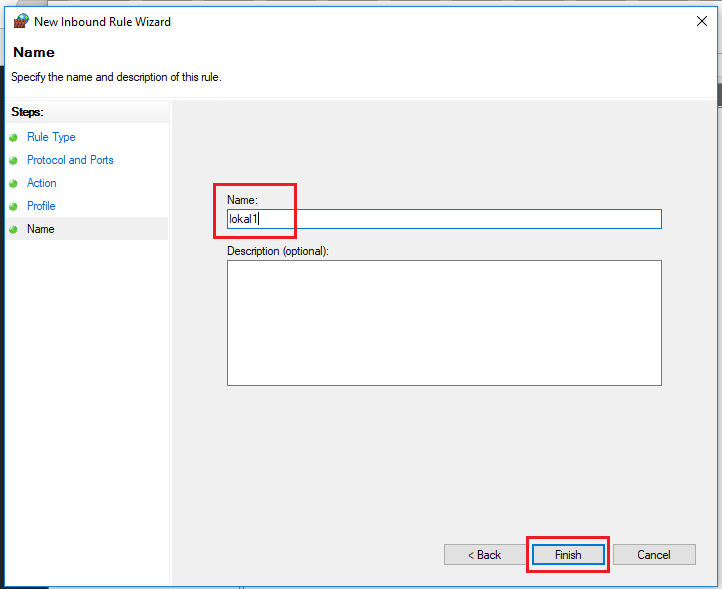
\includegraphics[width=0.7\textwidth]{figures/XAMPP/Xampp19.png}
    		\label{Xampp19}
		\end{figure}
		
	\item Ulangi kembali langkah 1 sampai 6, untuk langkah 6 isi dengan lokal2, kemudian klik Finish
	
	\item Restart komputer Anda 
\end{enumerate}

\chapter{CODEIGNITER VERSI 4 BETA}
Codeigniter adalah sebuah framework untuk web yang dibuat dalam format PHP. Format yang dibuat ini selanjutnya dapat digunakan untu membuat sistem aplikasi web yang kompleks. Codeigniter dapat mempercepat proses pembuatan web, karena semua class dan modul yang dibutuhkan sudah ada dan programmer hanya tinggal menggunakannya kembali pada aplikasi web yang akan dibuat \cite{prabowo2015website}.

\section{Tutorial Install CodeIgniter 4}
\label{carainstallci4}
    \begin{enumerate}
        \item Kunjungi Link Resmi CodeIgniter di \textbf{\textit{"https://www.codeigniter.com/download"}}, kemudian pilih menu "View CodeIgniter 4 on Github".
		\begin{figure}[!htbp]
    		\centering
    		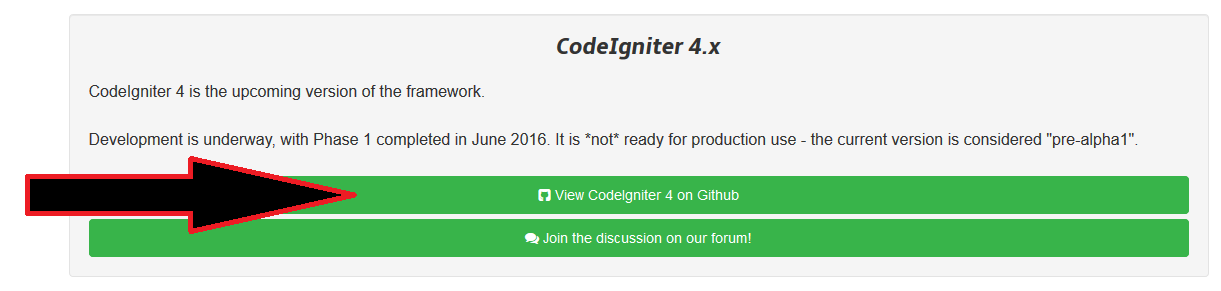
\includegraphics[width=0.9\textwidth]{figures/CODEIGNITER4/CI1_1.png}
    		\label{CodeIgniter1}
		\end{figure}
		
		\item Anda akan dibawa ke web github, dimana terdapat repository resmi untuk pengembangan Framework CodeIgniter 4, klik “Clone or download” kemudian “Download ZIP” untuk melakukan download Framework CodeIgniter 4.
		\begin{figure}[!htbp]
    		\centering
    		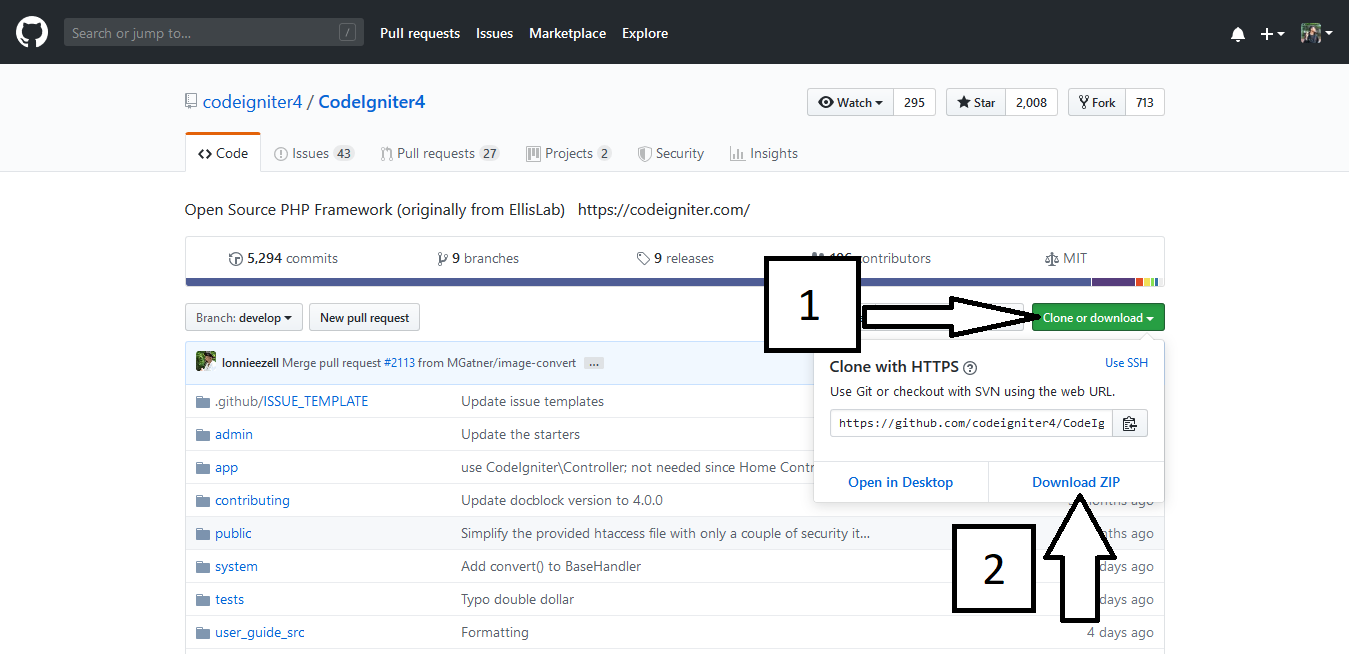
\includegraphics[width=0.5\textwidth]{figures/CODEIGNITER4/CI2.png}
    		\label{CodeIgniter2}
		\end{figure}
		
		\item Tunggu proses download sampai selesai, kemudian buka lokasi file yang didownload tadi dan copy file CodeIgniter4 ke dalam folder Xampp yang sudah di install sebelumnya di \verb|“C:\xampp7\htdocs”|.
		
		\item Extract file di folder tersebut, kemudian rename foldernya dengan nama aplikasi yang akan anda bangun, disini saya melakukan penamaan foldernya menjadi \verb|“ci4_leafletjs”|.
		\begin{figure}[!htbp]
    		\centering
    		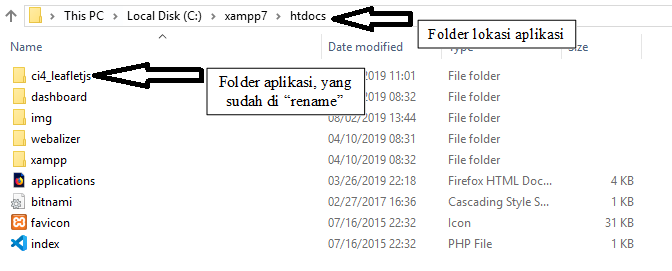
\includegraphics[width=0.5\textwidth]{figures/CODEIGNITER4/CI3.PNG}
    		\label{CodeIgniter3}
		\end{figure}
		
		\item Buka aplikasi \verb|“ci4_leafletjs”| dengan editor kesayangan anda, disini saya menggunakan visual studio code. Cara instal dan download bisa mengunjungi link berikut: \textbf{\textit{"https://code.visualstudio.com/download"}}.
		\begin{figure}[!htbp]
    		\centering
    		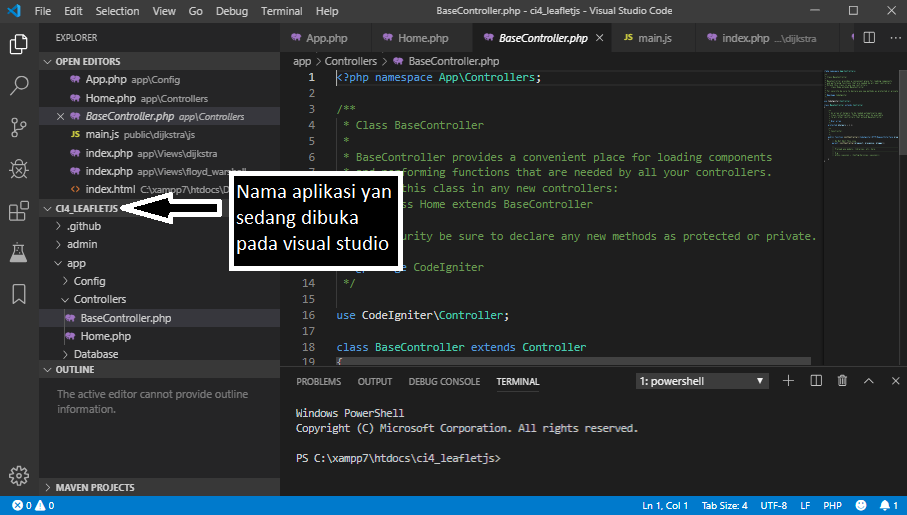
\includegraphics[width=0.5\textwidth]{figures/CODEIGNITER4/CI4.PNG}
    		\label{CodeIgniter4}
		\end{figure}
		
		\item Buka file App.php pada folder "app/Config/App.php", kemudian pada bagian \verb|"public $baseURL = ''"| diganti menjadi link aplikasi, sehingga seperti ini \verb|"public $baseURL = 'http://localhost:8080/';"|.
		\begin{figure}[!htbp]
    		\centering
    		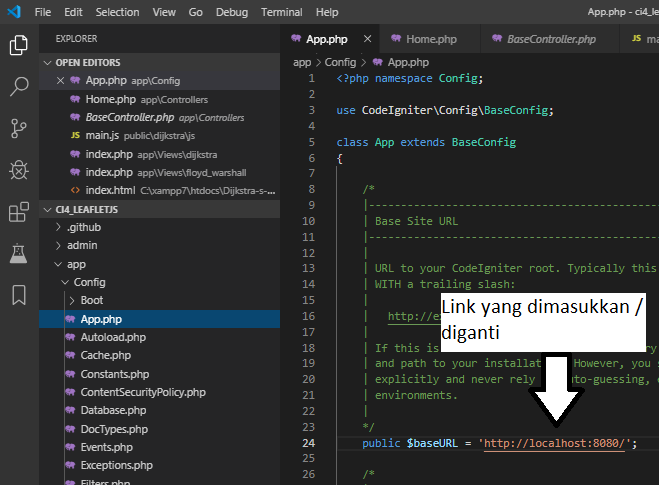
\includegraphics[width=0.5\textwidth]{figures/CODEIGNITER4/CI5.PNG}
    		\label{CodeIgniter5}
		\end{figure}
		
		\item CodeIgniter 4 sudah siap digunakan, jalankan aplikasi tersebut dengan cara berikut:
		\label{cararunci4}
		\begin{enumerate}
		    \item Klik menu Terminal yang ada pada menu bar atas Visual Studio Code, kemudian klik New Terminal atau bisa dengan cara menekan "Ctrl + Shift + `" pada keyboard anda. Setelah itu akan muncul terminal dibagian bawah pada Visual Studio Code seperti pada gambar berikut:
    		\begin{figure}[!htbp]
        		\centering
        		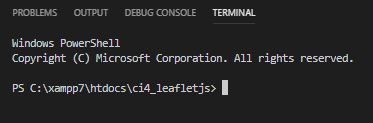
\includegraphics[width=0.5\textwidth]{figures/CODEIGNITER4/CI6.PNG}
        		\label{CodeIgniter6}
    		\end{figure}
    		
    		\item Masuk ke dalam folder public dengan cara mengetikkan "cd public" pada terminal.
    		\begin{figure}[!htbp]
        		\centering
        		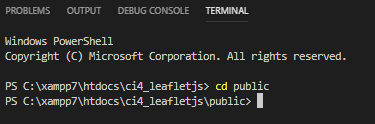
\includegraphics[width=0.5\textwidth]{figures/CODEIGNITER4/CI7.PNG}
        		\label{CodeIgniter7}
    		\end{figure}
    		
    		\item Ketikkan "php -S localhost:8080" pada terminal sehingga terlihat seperti pada gambar berikut:
    		\begin{figure}[!htbp]
        		\centering
        		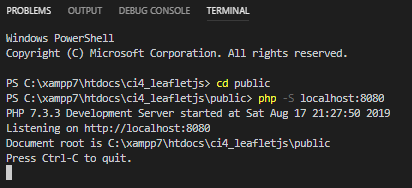
\includegraphics[width=0.5\textwidth]{figures/CODEIGNITER4/CI8.PNG}
        		\label{CodeIgniter8}
    		\end{figure}
    		
    		\item Bisa juga menggunakan cara kedua yaitu dengan mengetikkan "php spark serve" pada terminal sehingga terlihat seperti pada gambar berikut:
    		\begin{figure}[!htbp]
        		\centering
        		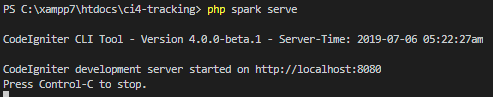
\includegraphics[width=0.5\textwidth]{figures/CODEIGNITER4/CI8_1.PNG}
        		\label{CodeIgniter9}
    		\end{figure}
    		
    		\item Jalankan aplikasi \verb|ci4_leafletjs| anda pada browser kesayangan anda, dengan cara mengetikkan "localhost:8080".
    		\begin{figure}[!htbp]
        		\centering
        		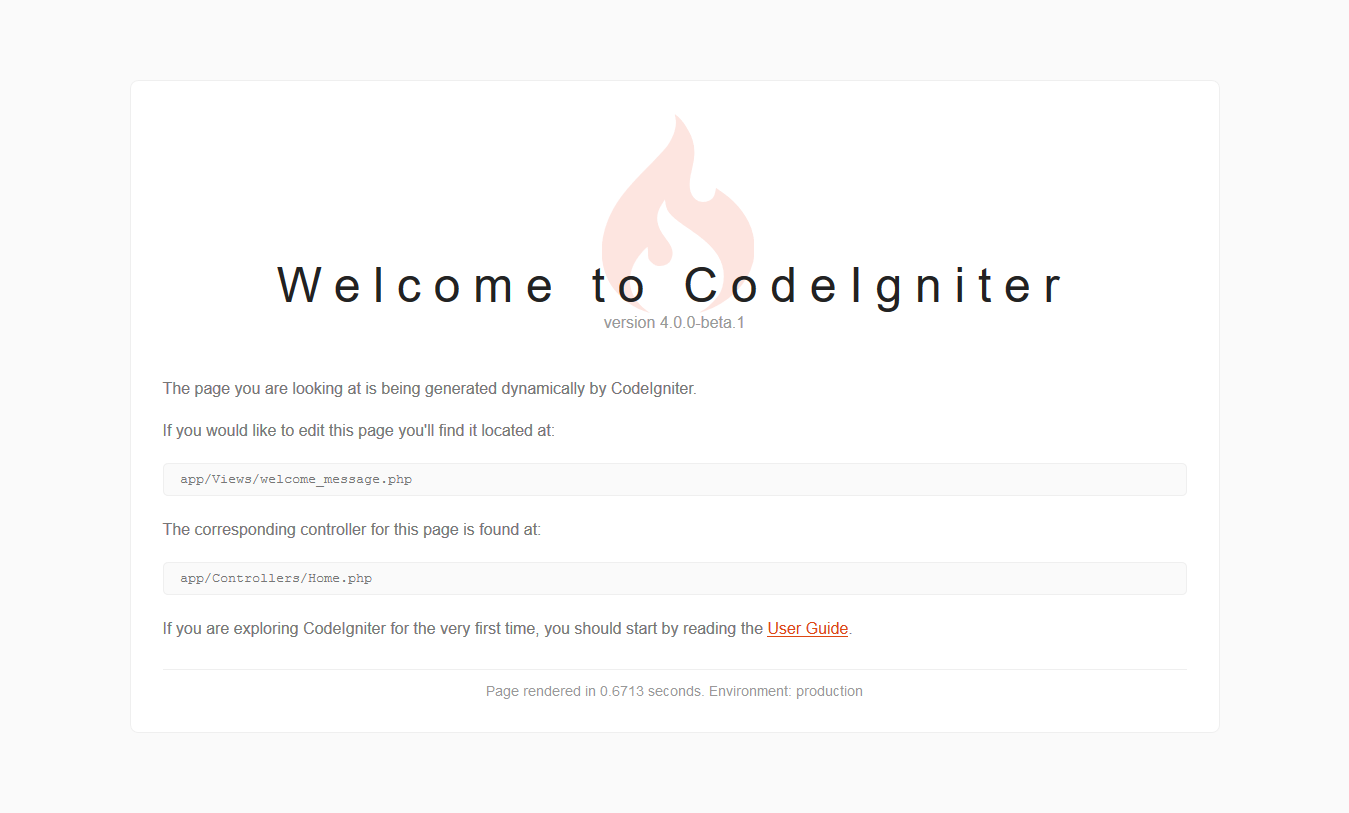
\includegraphics[width=0.8\textwidth]{figures/CODEIGNITER4/CI9.png}
        		\label{CodeIgniter10}
    		\end{figure}
    		
    		\item Kenapa "localhost:8080"? karena CodeIgniter 4 dilengkapi dengan server pengembangan lokal, memanfaatkan server web bawaan PHP dengan perutean CodeIgniter. Untuk info lebih jelasnya dapat dilihat pada link \textbf{\textit{"https:/ /codeigniter4.github.io/userguide/installation/running.html"}}.
		\end{enumerate}
    \end{enumerate}
    
    
    
    
    
\section{Konfigurasi CodeIgniter 4}
Di dalam folder config pada CodeIgniter terdapat berbagai macam file konfigurasi yang dapat kita atur sendiri nantinya. File tersebut dapat ditemukan pada folder \verb|C:/xampp7/htdocs/ci4_leafletjs/app/Config/|. Untuk codeigniter 4 default konfigurasi bisa dilakukan pada 3 file yaitu, file App.php, Database.php dan Routes.php. Berikut cara konfigurasinya:
\begin{enumerate}
    \item \textbf{App.php}, digunakan untuk membuat pengaturan dasar untuk web app codeigniter anda, seperti \verb|base_url|, index page, cookie, proxy dan lain lain. Configurasi pada file ini dapat dilakukan sama seperti pada configurasi sebelumnya di section 2.1
    \item \textbf{Database.php}, digunakan untuk mengatur koneksi web app kita ke database. Pada database.php konfigurasi yang dilakukan untuk mengkoneksikan database yaitu MySQL dengan aplikasi web berbasis framework CodeIgniter.
    \item \textbf{Routes.php}, digunakan untuk mengatur default controller dan overide 404.
\end{enumerate}





\section{Konfigurasi Template CodeIgniter 4}
Ada berbagai macam konfigurasi template terhadap CodeIgniter, baik secara install maupun dengan cara konfigurasi sendiri. Pada tutorial kali ini saya ingin menerapkan bootstrap dan template di CodeIgniter dengan cara cepat. Untuk yang ingin menggunakan cara instan, bisa dengan cara mengunjungi website \textit{w3layout.com} dan website yang menyediakan assets template dan bootstrap siap pakai. Sedikit berbeda dengan codeigniter 3 yang dimana harus dibuatkan folder assets terlebih dahulu, untuk codeigniter 4 semua assets akan ditampung dalam satu folder yaitu folder public, dapat di temukan pada folder \verb|C:\xampp7\htdocs\ci4_leafletjs\public|, berikut cara konfigurasi template pada codeigniter 4:
\begin{enumerate}
    \item Siapkan template atau bootstrap yang sudah didownload
    \item Extrak file tersebut jika dalam bentuk .rar atau .zip
    \item Copy file hasil extrak tadi ke dalam folder public.
		\begin{figure}[!htbp]
    		\centering
    		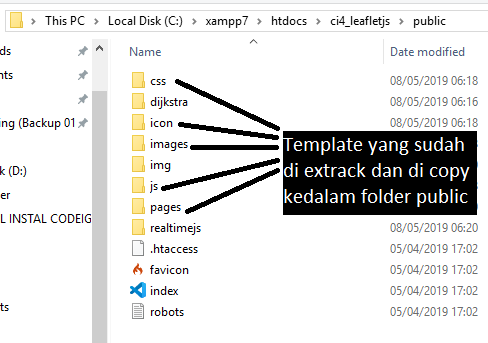
\includegraphics[width=0.5\textwidth]{figures/CODEIGNITER4/CI10.PNG}
    		\label{CodeIgniter11}
		\end{figure}
		
	\item Setelah menkopi file kedalam folder public, langka selanjutnya adalah memanggil config tersebut. Jangan lupa untuk membuat header dan footer ketika membuat website guna untuk mempermudah apabila terjadi perubahan terhadap beberapa menu.
	\item Copy isi dari index.html yang ada dalam template kemudian buat file di dalam folder \verb|C:/xampp7/htdocs/ci4_leafletjs/app/|views/agoritma/ index.php dengan format .php dan pastekan dalam file tersebut.
	\item Pertama lakukan konfigurasi terhadap index.php dengan cara memanggil link dan script yang sudah di copy di dalam folder public, berikut contoh pemanggilanya:
\begin{lstlisting}[caption=Konfigurasi Template di CodeIgniter 4]
<!DOCTYPE html>
<html lang="en">

<head>
    <meta charset="utf-8">
    <meta name="viewport" content="width=device-width, initial-scale=1.0, user-scalable=0, minimal-ui">
    <meta http-equiv="X-UA-Compatible" content="IE=edge" />
    <meta name="description" content="CodedThemes">
    <meta name="keywords" content=" Admin , Responsive, Landing, Bootstrap, App, Template, Mobile, iOS, Android, apple, creative app">
    <meta name="author" content="CodedThemes">

    <title>Dijkstra's Algorithm and Floyd-Warshall Algorithm</title>
  
    <link rel="icon" type="image/png" href="/images/favicon-32x32.png" sizes="32x32" />
    <link rel="icon" type="image/png" href="/images/favicon-16x16.png" sizes="16x16" />
    <link rel="icon" href="/images/favicon.ico" type="image/x-icon">
    <link rel="stylesheet" type="text/css" href="/css/bootstrap/css/bootstrap.min.css">
    <link rel="stylesheet" type="text/css" href="/css/datatables.css">
    <link rel="stylesheet" type="text/css" href="/css/buttons.dataTables.min.css">
    <link rel="stylesheet" type="text/css" href="/css/select2.css">
    <link rel="stylesheet" type="text/css" href="/css/style.css">
    <link rel="stylesheet" type="text/css" href="/css/style-bulog.css">
    <link rel="stylesheet" type="text/css" href="/css/style-bulog-print.css" media="print">
    <link rel="stylesheet" type="text/css" href="/css/jquery.mCustomScrollbar.css">
    <script type="text/javascript" src="/js/jquery/jquery.min.js"></script>
</head>
<body>
.....
    <div class="pcoded-content">
      <div class="pcoded-inner-content">
        <div class="main-body">
          <div class="page-wrapper">
            <div class="page-header card">
              <div class="row align-items-start">
                <div class="col-lg-8">
                  <div class="page-header-title">        
                    &copy; Faisal Syarifuddin <?php echo date('Y') ?>
                    <br>CodeIgniter Version <?= CodeIgniter\CodeIgniter::CI_VERSION ?>
                  </div>
                </div>
              </div>
            </div>
          </div>
        </div>
      </div>
    </div>
  </div>
  <script type="text/javascript" src="/js/script.js"></script>
</body>
</html>
\end{lstlisting}
		\par Lakukan pemanggilan terhadap semua code yang berbau href dan src, seperti pada codingan diatas. Setelah itu simpan.
		
	\item Pemanggilan template sudah selesai, jalankan aplikasi seperti pada cara yang sudah diterapakan sebelumnya di subbab \ref{carainstallci4}, maka akan muncul tampilan seperti gambar berikut:
		\begin{figure}[!htbp]
    		\centering
    		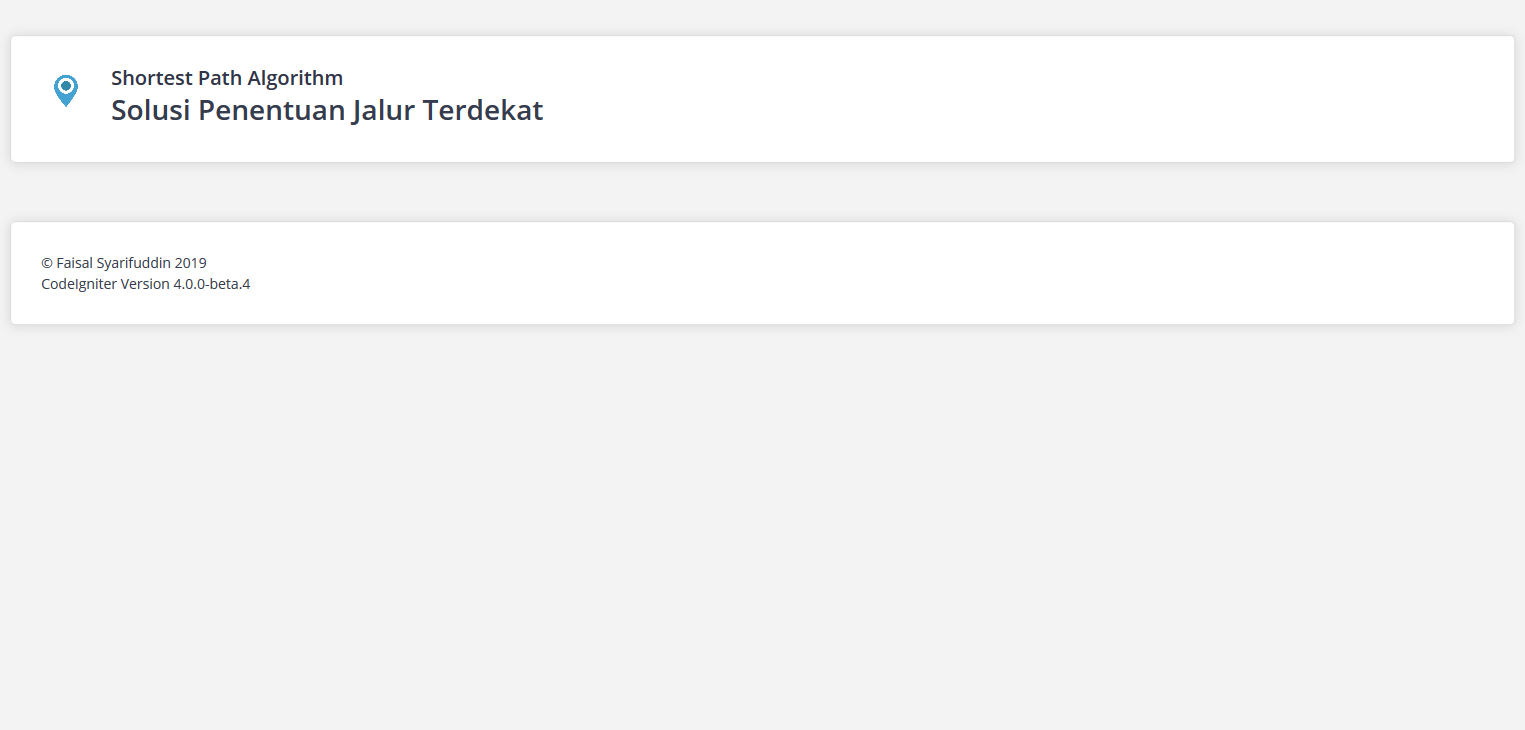
\includegraphics[width=0.8\textwidth]{figures/CODEIGNITER4/CI11.png}
    		\label{CodeIgniter12}
		\end{figure}
\end{enumerate}

\chapter{LEAFLET JS}
Leaflet adalah pustaka JavaScript open-source terkemuka untuk peta interaktif ramah-mobile. Dengan berat hanya sekitar 38 KB JS, ia memiliki semua fitur pemetaan yang paling dibutuhkan pengembang. Leaflet dirancang dengan kesederhanaan, kinerja, dan kegunaan dalam pikiran. Ini bekerja secara efisien di semua platform desktop dan seluler utama, dapat diperluas dengan banyak plugin, memiliki API yang indah, mudah digunakan dan didokumentasikan dengan baik dan kode sumber yang mudah dibaca dan menyenangkan untuk berkontribusi \cite{everviewleaflet}.


\section{Cara Menampilkan Map Leaflet JS di CodeIgniter}
\begin{enumerate}
    \item Buka salah satu file php yang ingin Anda berikan fitur map, file dapat ditemukan ada pada folder  \verb|C:/xampp7/htdocs/ci4_leafletjs/app/Views/|.
    \item Pada bagian \verb|<head>| sertakan file Leaflet CSS.
\begin{lstlisting}[caption=File Leaflet CSS]
<head>
    <meta charset="utf-8">
    <meta name="viewport" content="width=device-width, initial-scale=1.0, user-scalable=0, minimal-ui">
    <meta http-equiv="X-UA-Compatible" content="IE=edge" />
    <meta name="description" content="CodedThemes">
    <meta name="keywords" content=" Admin , Responsive, Landing, Bootstrap, App, Template, Mobile, iOS, Android, apple, creative app">
    <meta name="author" content="CodedThemes">
    
    <link rel="stylesheet" href="https://unpkg.com/leaflet@1.5.1/dist/leaflet.css"integrity="sha512-xwE/Az9zrjBIphAcBb3F6JVqxf46+CDLwfLMHloNu6KEQCAWi6HcDUbeOfBIptF7tcCzusKFjFw2yuvEpDL9wQ=="crossorigin=""/>
</head>
.....
\end{lstlisting}

    \item Kemudian sertakan file JavaScript Leaflet setelah CSS Leaflet, pada  bagian footer atau sebelum penutup \verb|</body>|.
\begin{lstlisting}[caption=File JavaScript Leaflet]
.....
    <script src="https://unpkg.com/leaflet@1.5.1/dist/leaflet.js"integrity="sha512-GffPMF3RvMeYyc1LWMHtK8EbPv0iNZ8/oTtHPx9/cc2ILxQ+u905qIwdpULaqDkyBKgOaB57QTMg7ztg8Jm2Og=="crossorigin=""></script>

</body>
</html>
\end{lstlisting}

    \item Map sudah siap untuk ditampilkan, selanjutnya adalah meletakkan elemen div dengan id tertentu di mana Anda ingin peta Anda berada.
\begin{lstlisting}[caption=Elemen div map Leaflet]
.....
    <div id="mapid"></div>
.....
\end{lstlisting}

    \item Jalankan aplikasi kemudian akan tampil map seperti berikut:
	\begin{figure}[!htbp]
		\centering
		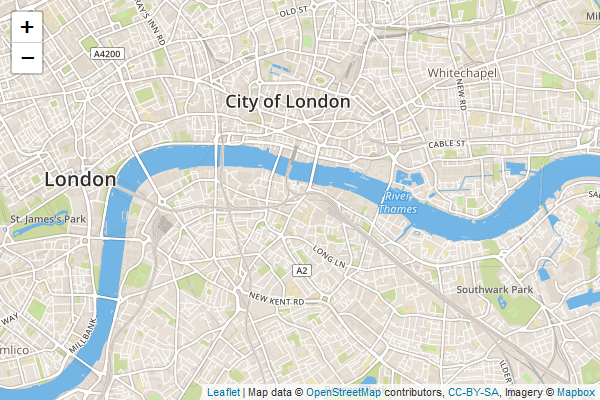
\includegraphics[width=0.5\textwidth]{figures/LEAFLETJS/LJS1.png}
		\label{Leaflet1}
	\end{figure}
\end{enumerate}





\section{Menampilkan Mapbox Pada index.php} 
\label{7.2}
Pada bab sebelumnya sudah dilakukan konfigurasi beberapa template untuk mepercantik tampilan index.php. Kemudian selanjutnya adalah bagaimana cara memasang mapbox pada index.php? Berikut caranya:
\begin{enumerate}
    \item Tambahkan config pada bagian head dan footer index.php dapat dilihat seperti pada codingan dibawah ini:

\begin{lstlisting}[caption=Menampilkan Mapbox Leaflet JS di CodeIgniter 4]
.....
<head>
    <link href="/algoritma/style/justified-nav.css" rel="stylesheet">
    <link href="https://fonts.googleapis.com/css?family=Open+Sans:400,600" rel="stylesheet">
    <link rel="stylesheet" href="https://unpkg.com/leaflet@1.3.1/dist/leaflet.css" integrity="sha512-Rksm5RenBEKSKFjgI3a41vrjkw4EVPlJ3+OiI65vTjIdo9brlAacEuKOiQ5OFh7cOI1bkDwLqdLw3Zg0cRJAAQ==" crossorigin=""/>
</head>
.....
  <script src="https://code.jquery.com/jquery-3.2.1.min.js"></script>
  <script src="https://cdnjs.cloudflare.com/ajax/libs/popper.js/1.11.0/umd/popper.min.js" integrity="sha384-b/U6ypiBEHpOf/4+1nzFpr53nxSS+GLCkfwBdFNTxtclqqenISfwAzpKaMNFNmj4" crossorigin="anonymous"></script>
  <script src="https://maxcdn.bootstrapcdn.com/bootstrap/4.0.0-beta/js/bootstrap.min.js" integrity="sha384-h0AbiXch4ZDo7tp9hKZ4TsHbi047NrKGLO3SEJAg45jXxnGIfYzk4Si90RDIq Nm1" crossorigin="anonymous"></script>
  <script src="https://cdn.jsdelivr.net/npm/d3@3.3.0/d3.min.js"></script>
  
  <script src="https://cdn.jsdelivr.net/npm/leaflet@0.7.7/dist/leaflet.js"></script>

  <script src="/algoritma/js/main.js"></script>
  <script src="/algoritma/js/ie10-viewport-bug-workaround.js"></script>
 .....
\end{lstlisting}

    \item Kemudian pada folder \verb|C:\xampp7\htdocs\ci4_leafletjs\public|, buat satu folder dengan nama algoritma dimana dalam folder ini akan di masukkan beberapa js tentang algoritma dijkstra dan floyd warshall dan js tentang package leaflet.
    \vspace{5cm}
	\begin{figure}[!htbp]
		\centering
		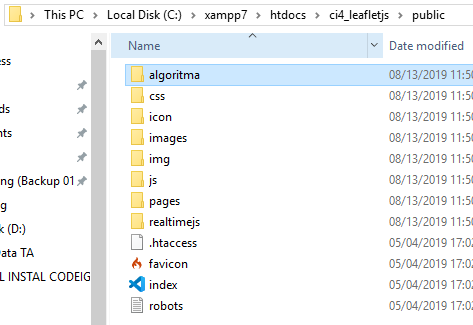
\includegraphics[width=0.5\textwidth]{figures/LEAFLETJS/LJS2.PNG}
		\label{Leaflet2}
	\end{figure}
	
	\item Buka folder algoritma kemudian buat folder dengan nama js dan buat file didalam folder js dengan nama main.js. Dalam file ini nantinya tersimpan beberapa konfigurasi seperti konfigurasi untuk leaflet js dan algoritma yang akan digunakan dalam penentuan rute terdekat.
	
	\item Buka file main.js kemudian isikan kodingan berikut:
\begin{lstlisting}[caption=Setting setView Pada Leaflet JS]
var graphmap, svg, maps, g;

var mapdata = {
    allnodes: [],
    paths: [],
    distances: [],
    getui: {
        htmlSelectStartingNode: "#from-starting",
        htmlSelectEndNode: "#to-end"
    },
    getstate: {
        selectedNode: null,
        fromNode: null,
        toNode: null
    }
};

maps = L.map('svg-map').setView([-6.8731953,107.5737873,17], 15);
//Menampilkan lokasi maps politeknik pos indonesia dengan max zoom 15 saat pertama kali load aplikasi
mapLink = '<a href="http://openstreetmap.org">OpenStreetMap</a>';
L.tileLayer('https://api.tiles.mapbox.com/v4/{id}/{z}/{x}/{y}.png?access_token={accessToken}', {
    attribution: 'Map data &copy; <a href="http://openstreetmap.org">OpenStreetMap</a> contributors, <a href="http://creativecommons.org/licenses/by-sa/2.0/">CC-BY-SA</a>, Imagery © <a href="http://mapbox.com">Mapbox</a>',
    maxZoom: 18,
    id: 'mapbox.streets',
    accessToken: 'pk.eyJ1IjoiaW1hZHVkZGluaGFyaXMiLCJhIjoiY2p1d2E3MzM4MGFiZDRkcGYyM WF3emtlYiJ9.KTemDE4IAujR0X-ltttotg'
}).addTo(maps);
maps._initPathRoot()
svg = d3.select("#svg-map").select("svg")
    .attr("class", "svgmap")
    .on("contextmenu", function () { d3.event.preventDefault(); })
\end{lstlisting}

    \item Simpan, kemudian panggil library js dalam index.php
\begin{lstlisting}[caption=Call Library setView]
<script src="/algoritma/js/main.js"></script>
\end{lstlisting}

    \item Berikut codingan full untuk tampilan index.php

\begin{lstlisting}[caption=Pemanggilan Library setView pada index.php]
<!DOCTYPE html>
<html lang="en">

<head>
    <meta charset="utf-8">
    <meta name="viewport" content="width=device-width, initial-scale=1.0, user-scalable=0, minimal-ui">
    <meta http-equiv="X-UA-Compatible" content="IE=edge" />
    <meta name="description" content="CodedThemes">
    <meta name="keywords" content=" Admin , Responsive, Landing, Bootstrap, App, Template, Mobile, iOS, Android, apple, creative app">
    <meta name="author" content="CodedThemes">
  <title>Shortest Path Algorithm</title>
  
  <link rel="stylesheet" href="https://maxcdn.bootstrapcdn.com/bootstrap/4.0.0-beta/css/bootstrap.min.css" integrity="sha384-/Y6pD6FV/Vv2HJnA6t+vslU6fwYXjCFtcEpHbNJ0lyAFsXTsjBbfaDjzALeQsN6M" crossorigin="anonymous">
  <link href="/algoritma/style/justified-nav.css" rel="stylesheet">
  
    <link rel="icon" type="image/png" href="/images/favicon-32x32.png" sizes="32x32" />
    <link rel="icon" type="image/png" href="/images/favicon-16x16.png" sizes="16x16" />
    <link rel="icon" href="/images/favicon.ico" type="image/x-icon">
    <link href="https://fonts.googleapis.com/css?family=Open+Sans:400,600" rel="stylesheet">
    <link rel="stylesheet" type="text/css" href="/css/bootstrap/css/bootstrap.min.css">
    <link rel="stylesheet" type="text/css" href="/icon/themify-icons/themify-icons.css">
    <link rel="stylesheet" type="text/css" href="/icon/icofont/css/icofont.css">
    <link rel="stylesheet" type="text/css" href="/css/datatables.css">
    <link rel="stylesheet" type="text/css" href="/css/buttons.dataTables.min.css">
    <link rel="stylesheet" type="text/css" href="/css/select2.css">
    <link rel="stylesheet" type="text/css" href="/css/style.css">
    <link rel="stylesheet" type="text/css" href="/css/style-bulog.css">
    <link rel="stylesheet" type="text/css" href="/css/style-bulog-print.css" media="print">
    <link rel="stylesheet" type="text/css" href="/css/jquery.mCustomScrollbar.css">
    <link rel="stylesheet" href="https://cdnjs.cloudflare.com/ajax/libs/font-awesome/4.7.0/css/font-awesome.min.css">

    <script type="text/javascript" src="/js/jquery/jquery.min.js"></script>
    <link rel="stylesheet" href="https://unpkg.com/leaflet@1.3.1/dist/leaflet.css" integrity="sha512-Rksm5RenBEKSKFjgI3a41vrjkw4EVPlJ3+OiI65vTjIdo9brlAacEuKOiQ5OFh7cOI1bkDwLqdLw3Zg0cRJAAQ==" crossorigin=""/>
</head>
<body>
    <div class="theme-loader">
      <div class="ball-scale">
        <img src="/images/logo-track.png"/>
      </div>
    </div>

    <div class="loading-wrap">
      <div class="loading-box">
        <img src="/images/logo-track.png"/>
        <span>Mohon tunggu...</span>
        <div class="progress" style="height: 10px;">
          <div id="progress-bar" class="progress-bar" role="progressbar"></div>
        </div>
      </div>
    </div>

    <div class="pcoded-content">
      <div class="pcoded-inner-content">
        <div class="main-body">
          <div class="page-wrapper">
            <div class="page-header card">
              <div class="row align-items-start">
                <div class="col-lg-12">
                  <div class="page-header-title">
                    <div class="icon-logo">
                      <img src="/images/logo-track.png"/>
                    </div>
                    <div class="d-inline">
                      <h4 class="m-b-15 block">Shortest Path Algorithm</h4>
                      <h3 class="m-t-5"><strong>Solusi Penentuan Jalur Terdekat</strong></h3>
                    </div>
                  </div>
                </div>
              </div>
            </div>
            <br />
          </div>
        </div>
      </div>
    </div>

    <div class="row">
      <div class="col-lg-12">
        <div id="svg-map" style="width: 1110px; height: 800px" class="card">
        </div>
      </div>
    </div>

    <div class="pcoded-content">
      <div class="pcoded-inner-content">
        <div class="main-body">
          <div class="page-wrapper">
            <div class="page-header card">
              <div class="row align-items-start">
                <div class="col-lg-8">
                  <div class="page-header-title">        
                    &copy; Faisal Syarifuddin <?php echo date('Y') ?>
                    <br>CodeIgniter Version <?= CodeIgniter\CodeIgniter::CI_VERSION ?>
                  </div>
                </div>
              </div>
            </div>
          </div>
        </div>
      </div>
    </div>
  </div>

  <script src="https://code.jquery.com/jquery-3.2.1.min.js"></script>
  <script src="https://cdnjs.cloudflare.com/ajax/libs/popper.js/1.11.0/umd/popper.min.js" integrity="sha384-b/U6ypiBEHpOf/4+1nzFpr53nxSS+GLCkfwBdFNTxtclqqenISfwAzpKaMNFNmj4" crossorigin="anonymous"></script>
  <script src="https://maxcdn.bootstrapcdn.com/bootstrap/4.0.0-beta/js/bootstrap.min.js" integrity="sha384-h0AbiXch4ZDo7tp9hKZ4TsHbi047NrKGLO3SEJAg45jXxnGIfYzk4Si90RDIq Nm1" crossorigin="anonymous"></script>
  <script src="https://cdn.jsdelivr.net/npm/d3@3.3.0/d3.min.js"></script>
  <script src="https://cdn.jsdelivr.net/npm/leaflet@0.7.7/dist/leaflet.js"></script>
  <script src="/algoritma/js/main.js"></script>
  <script src="/algoritma/js/ie10-viewport-bug-workaround.js"></script>
  <script type="text/javascript" src="/js/script.js"></script>

</body>
</html>
\end{lstlisting}

    \item Simpan file index.php tersebut kemudian jalankan aplikasi anda, maka pada browser aka muncup map box seperti pada gambar berikut.
	\begin{figure}[!htbp]
		\centering
		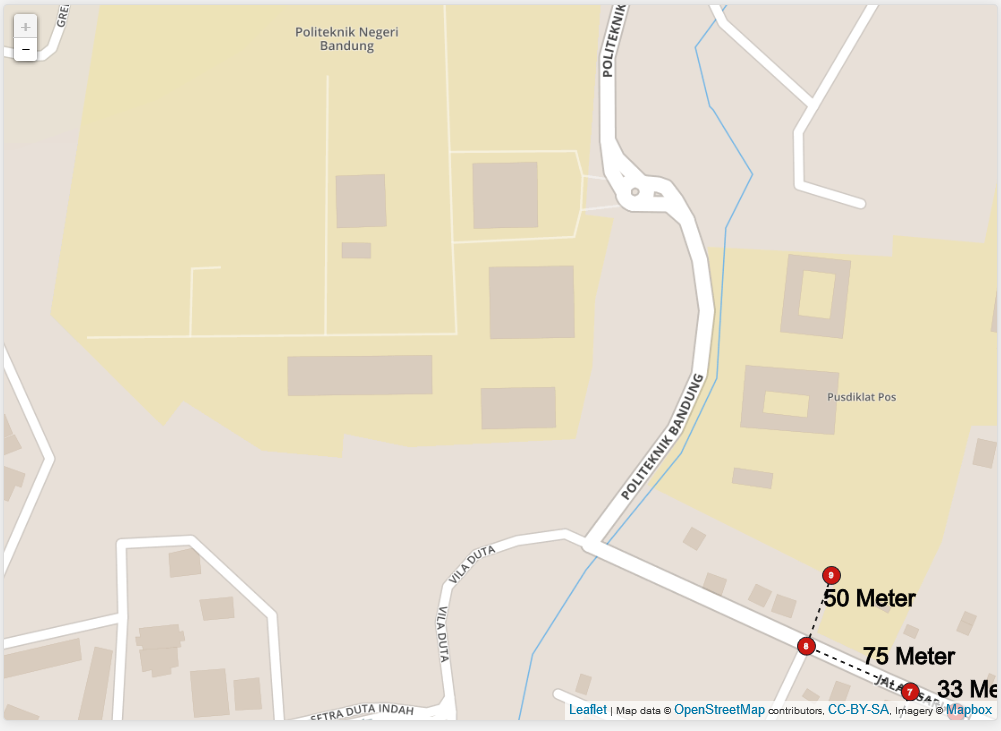
\includegraphics[width=0.5\textwidth]{figures/LEAFLETJS/LJS3.png}
		\label{Leaflet3}
	\end{figure}

\end{enumerate}




\section{Penetuan Jalur Terdekat Dengan Algoritma Dijkstra dan Floyd Warshal}
Melanjutnkan Kodingan sebelumnya, pada tahap ini anda akan membuat UI, dan beberapa function yang untuk algoritma dijsktra dan floyd warshal. Berikut tahapan membuat sistem penentuan jalur terdekat menggunakan algoritma dijsktra dan floyd warshall:
\begin{enumerate}
    \item Membuat index.php pada folder algoritma (Sebelumnya sudah di buat pada point \ref{7.2}).
    \item Melengkapi library yang ada pada index.php pada point \ref{7.2}, seperti pada kodingan dibawah:
\begin{lstlisting}[caption=index.php Full Code]
<!DOCTYPE html>
<html lang="en">

<head>
    <meta charset="utf-8">
    <meta name="viewport" content="width=device-width, initial-scale=1.0, user-scalable=0, minimal-ui">
    <meta http-equiv="X-UA-Compatible" content="IE=edge" />
    <meta name="description" content="CodedThemes">
    <meta name="keywords" content=" Admin , Responsive, Landing, Bootstrap, App, Template, Mobile, iOS, Android, apple, creative app">
    <meta name="author" content="CodedThemes">

  <title>Shortest Path Algorithm</title>
  <link rel="stylesheet" href="https://maxcdn.bootstrapcdn.com/bootstrap/4.0.0-beta/css/bootstrap.min.css" integrity="sha384-/Y6pD6FV/Vv2HJnA6t+vslU6fwYXjCFtcEpHbNJ0lyAFsXTsjBbfaDjzALeQsN6M" crossorigin="anonymous">
  <link href="/algoritma/style/justified-nav.css" rel="stylesheet">
  
    <link rel="icon" type="image/png" href="/images/favicon-32x32.png" sizes="32x32" />
    <link rel="icon" type="image/png" href="/images/favicon-16x16.png" sizes="16x16" />
    <link rel="icon" href="/images/favicon.ico" type="image/x-icon">
    <link href="https://fonts.googleapis.com/css?family=Open+Sans:400,600" rel="stylesheet">
    <link rel="stylesheet" type="text/css" href="/css/bootstrap/css/bootstrap.min.css">
    <link rel="stylesheet" type="text/css" href="/icon/themify-icons/themify-icons.css">
    <link rel="stylesheet" type="text/css" href="/icon/icofont/css/icofont.css">
    <link rel="stylesheet" type="text/css" href="/css/datatables.css">
    <link rel="stylesheet" type="text/css" href="/css/buttons.dataTables.min.css">
    <link rel="stylesheet" type="text/css" href="/css/select2.css">
    <link rel="stylesheet" type="text/css" href="/css/style.css">
    <link rel="stylesheet" type="text/css" href="/css/style-bulog.css">
    <link rel="stylesheet" type="text/css" href="/css/style-bulog-print.css" media="print">
    <link rel="stylesheet" type="text/css" href="/css/jquery.mCustomScrollbar.css">
    <link rel="stylesheet" href="https://cdnjs.cloudflare.com/ajax/libs/font-awesome/4.7.0/css/font-awesome.min.css">

    <script type="text/javascript" src="/js/jquery/jquery.min.js"></script>
    <link rel="stylesheet" href="https://unpkg.com/leaflet@1.3.1/dist/leaflet.css" integrity="sha512-Rksm5RenBEKSKFjgI3a41vrjkw4EVPlJ3+OiI65vTjIdo9brlAacEuKOiQ5OFh7cOI1bkDwLqdLw3Zg0cRJAAQ==" crossorigin=""/>

</head>
<body>
    <div class="theme-loader">
      <div class="ball-scale">
        <img src="/images/logo-track.png"/>
      </div>
    </div>

    <div class="loading-wrap">
      <div class="loading-box">
        <img src="/images/logo-track.png"/>
        <span>Mohon tunggu...</span>
        <div class="progress" style="height: 10px;">
          <div id="progress-bar" class="progress-bar" role="progressbar"></div>
        </div>
      </div>
    </div>

    <div class="pcoded-content">
      <div class="pcoded-inner-content">
        <div class="main-body">
          <div class="page-wrapper">
            <div class="page-header card">
              <div class="row align-items-start">
                <div class="col-lg-12">
                  <div class="page-header-title">
                    <div class="icon-logo">
                      <img src="/images/logo-track.png"/>
                    </div>
                    <div class="d-inline">
                      <h4 class="m-b-15 block">Shortest Path Algorithm</h4>
                      <h3 class="m-t-5"><strong>Solusi Penentuan Jalur Terdekat</strong></h3>
                    </div>
                  </div>
                </div>
              </div>
            </div>
            <br />
          </div>
        </div>
      </div>
    </div>

  <div class="container">
    <div class="row">
      <div class="col-lg-12">
            <label class="mr-sm-2" for="from">Cara penggunaan: Tentukan titik-titik sesuai di maps dengan cara klik kiri, kemudian sambungkan titik satu dengan titik lainnya dengan cara klik kanan titik awal dan klik kanan titik tujuan, pilih route dari mana kemana di pilihan titik awal dan titik tujuan kemudian klik start route untuk melihat hasil algoritma sesuai tombol yg diklik.</label>

        <hr>
          <div class="form-row align-items-center">
            <div class="col-auto">
              <label class="mr-sm-2" for="from">Titik Awal : </label>
              <select id="from-starting" class="custom-select mb-2 mr-sm-2 mb-sm-0"></select>
            </div>

            <div class="col-auto">
              <label class="mr-sm-2" for="to">Titik Tujuan : </label>
              <select id="to-end" class="custom-select mb-2 mr-sm-2 mb-sm-0"></select>
            </div>

            <div class="col-auto">
              <button type="button" id="getshortestroute" class="btn btn-primary" title="find shortest path between nodes using dijkstra"><i class="fa fa-map-o" aria-hidden="true"> Start Dijkstra</i></button>
            </div>
            
            <div class="col-auto">
              <button type="button" id="floyd" class="btn btn-primary" title="find shortest path between nodes using floyd"><i class="fa fa-map-o" aria-hidden="true"> Start Floyd</i></button>
            </div>

            <div class="col-auto">
              <button type="button" id="clearmap" class="btn btn-danger"><i class="fa fa-trash-o" aria-hidden="true"> Hapus Map</i></button>
            </div>

            <div class="col-12">
              <br><br>
              <h6>Jalur terpendek: <span id="jtp"></span></h6>
            </div>
          </div>

      </div>
    </div>

    <div class="row">
      <div class="col-lg-12">
        <div id="svg-map" style="width: 1110px; height: 800px" class="card">
        </div>
      </div>
    </div>

    <hr>
    <form style="margin-top:5px;">
    <div class="form-row align-items-center">
      <div class="col-auto">
        <button type="button" class="btn btn-primary" id="data-export"> Export Data</button>
      </div>
    </div>
    </form>
    <hr>
    
    <div class="col-auto" style="margin-top: 5px;">
      <label class="mr-sm-2" for="inlineFormCustomSelect">Route Wisata Bandung</label>
      <select class="custom-select mb-2 mr-sm-2 mb-sm-0" id="setexample">
        <option value="0"></option>
        <option value="1">Titik Wisata Bandung</option>
        <option value="2">Data Titik Lokasi Wisata Bandung</option>
        <option value="3">Sample Data Politeknik Pos Indonesia</option>
        <option value="4">Dusun Bambu Lembang</option>
        <option value="5">Farmhouse Lembang</option>
        <option value="6">Gunung Tangkuban Perhau</option>
        <option value="7">Kebun Teh Sukawana</option>
        <option value="9">Tebing Kraton</option>
        <option value="10">Alun-Alun Bandung</option>
      </select>
    </div>
    <hr>

    <div class="pcoded-content">
      <div class="pcoded-inner-content">
        <div class="main-body">
          <div class="page-wrapper">
            <div class="page-header card">
              <div class="row align-items-start">
                <div class="col-lg-8">
                  <div class="page-header-title">        
                    &copy; Faisal Syarifuddin <?php echo date('Y') ?>
                    <br>CodeIgniter Version <?= CodeIgniter\CodeIgniter::CI_VERSION ?>
                  </div>
                </div>
              </div>
            </div>
          </div>
        </div>
      </div>
    </div>

  </div>

  <script src="https://code.jquery.com/jquery-3.2.1.min.js"></script>
  <script src="https://cdnjs.cloudflare.com/ajax/libs/popper.js/1.11.0/umd/popper.min.js" integrity="sha384-b/U6ypiBEHpOf/4+1nzFpr53nxSS+GLCkfwBdFNTxtclqqenISfwAzpKaMNFNmj4" crossorigin="anonymous"></script>
  <script src="https://maxcdn.bootstrapcdn.com/bootstrap/4.0.0-beta/js/bootstrap.min.js" integrity="sha384-h0AbiXch4ZDo7tp9hKZ4TsHbi047NrKGLO3SEJAg45jXxnGIfYzk4Si90RDIqNm1" crossorigin="anonymous"></script>
  <script src="https://cdn.jsdelivr.net/npm/d3@3.3.0/d3.min.js"></script>
  <script src="https://cdn.jsdelivr.net/npm/leaflet@0.7.7/dist/leaflet.js"></script>

  <script src="/algoritma/js/main.js"></script>
  <script src="/algoritma/js/ie10-viewport-bug-workaround.js"></script>
  <script type="text/javascript" src="/js/script.js"></script>

</body>
</html>
\end{lstlisting}

    \item Selanjutnya membuat function algoritma Dijkstra dan Floyd Warshall
    \begin{enumerate}
        \item Function Algoritma Dijsktra
    \begin{enumerate}
        \item Buka file main.js yang sudah dibuat sebelumnya pada point \ref{7.2} atau bisa ditemukan pada folder \verb|ci4_leafletjs\| kemudian dalam folder \verb|public\algoritma\js\main.js|.
        % C:\xampp7\htdocs\
        \item Buat functioin klik dijsktra pada main.js
\begin{lstlisting}[caption=Function OnClick Dijsktra]
$('#getshortestroute').on('click', function () {
    alert('Dijkstra');
    d3.selectAll("line").classed({ "shortest": false });
    calculateDistancesbetweennodes();
    if (!$(mapdata.getui.htmlSelectStartingNode).val() || !$(mapdata.getui.htmlSelectEndNode).val()) return;
    var sourceNode = $(mapdata.getui.htmlSelectStartingNode).val();
    var targetNode = $(mapdata.getui.htmlSelectEndNode).val();
    var results = dijkstra(sourceNode, targetNode);
    var distTotal = 0;
    var dist = null;
    var stepnode = '';
    if (results.path) {
        results.path.forEach(function (step) {

            dist = mapdata.distances[step.source][step.target]
            stepLine = d3.select(
                "line.from" + step.source + "to" + step.target + ","
                + "line.from" + step.target + "to" + step.source
            );
            stepLine.classed({ "shortest": true });
            stepnode += step.source+'->'+step.target+'->';
            distTotal = distTotal + dist;
        });
            var estimasiMenit = distTotal / 60; //perkiraan kecepatan 60 km/jam
            // var estimasiDetik = estimasiMenit * 3600 / 60;
            // var estimasiDetik = estimasiMenit * 60 / 3600;
            var estimasiDetik = (estimasiMenit - Math.floor(estimasiMenit)) * 60;
            var persentasilocaccuarcy = distTotal / 400;
                if(persentasilocaccuarcy <= 800){
                    persentasiloc = 'High';
                }else if(persentasilocaccuarcy >= 5000){
                    persentasiloc = 'Low';
                }else{
                    persentasiloc = 'Medium';
                }
            $('#jtp').html('(Dijkstra) '+Math.round(distTotal)+' m <br><br>Melewati node : start->'+stepnode+'end<br><br>Perkiraan waktu perjalanan: '+Math.round(estimasiMenit)+' menit, '+Math.round(estimasiDetik)+'detik<br><br>Persentasi Akurasi: '+persentasiloc+' ('+Math.round(persentasilocaccuarcy)+' %)');
    }

});
$('#clearmap').on('click', function () {
    clearGraph();
});
\end{lstlisting}
\label{FunctionOnClickDijsktra}
    \item Function ini akan di eksekusi ketika button pada index.php dengan id=getshortestroute di klik (button dijsktra).
\begin{lstlisting}[caption=Button Dijsktra]
<button type="button" id="getshortestroute" class="btn btn-primary" title="find shortest path between nodes using dijkstra">
\end{lstlisting}
\label{ButtonDijsktra}

    \item Selanjutnya membuat function dengan rumus dijsktra yang dihasilkan dari code listing psoudocode \ref{PseudocodeAlgoritmaDijkstra}. Function ini akan digunakan untuk mengeksekusi beberapa titik yang digunakan untuk menentukan jalur terdekat.
\begin{lstlisting}[caption=Function Algoritma Dijsktra]
function dijkstra(start, end) {
    var nodeCount = mapdata.distances.length,
        infinity = 99999, // infinity
        shortestPath = new Array(nodeCount),
        nodeChecked = new Array(nodeCount),
        pred = new Array(nodeCount);

    for (var i = 0; i < nodeCount; i++) {
        shortestPath[i] = infinity;
        pred[i] = null;
        nodeChecked[i] = false;
    }

    shortestPath[start] = 0;
    for (var i = 0; i < nodeCount; i++) {
        var minDist = infinity;
        var closestNode = null;
        for (var j = 0; j < nodeCount; j++) {
            if (!nodeChecked[j]) {
                if (shortestPath[j] <= minDist) {
                    minDist = shortestPath[j];
                    closestNode = j;
                }
            }
        }

        nodeChecked[closestNode] = true;
        for (var k = 0; k < nodeCount; k++) {
            if (!nodeChecked[k]) {
                var nextDistance = distanceBetween(closestNode, k, mapdata.distances);
                if ((parseInt(shortestPath[closestNode]) + parseInt(nextDistance)) < parseInt(shortestPath[k])) {
                    soFar = parseInt(shortestPath[closestNode]);
                    extra = parseInt(nextDistance);
                    shortestPath[k] = soFar + extra;
                    pred[k] = closestNode;
                }
            }
        }
    }

    if (shortestPath[end] < infinity) {
        var newPath = [];
        var step = {
            target: parseInt(end)
        };
        var v = parseInt(end);

        while (v >= 0) {
            v = pred[v];
            if (v !== null && v >= 0) {
                step.source = v;
                newPath.unshift(step);
                step = {
                    target: v
                };
            }
        }

        totalDistance = shortestPath[end];
        return {
            mesg: 'Status: OK',
            path: newPath,
            source: start,
            target: end,
            distance: totalDistance
        };
    } else {
        return {
            mesg: 'Sorry No path found',
            path: null,
            source: start,
            target: end,
            distance: 0
        };
    }

    function distanceBetween(fromNode, toNode, distances) {
        dist = distances[fromNode][toNode];
        if (dist === 'x') dist = infinity;
        return dist;
    }
};
\end{lstlisting}
\par Function ini akan di eksekusi ketika button dijsktra diklik, kemudian akan memanggil function dijsktra pada variable "var results = dijkstra(sourceNode, targetNode);" di function onclick button dijkstra.
    \end{enumerate}
    
    \item Function Algoritma Floyd Warshall
    \begin{enumerate}
        \item Masih di file main.js, buat functioin klik floyd warshal pada main.js
\begin{lstlisting}[caption=Function OnClick Dijsktra]
$('#floyd').on('click', function () {
    alert('Floyd Warshal');
    d3.selectAll("line").classed({ "shortest": false });
    calculateDistancesbetweennodes();
    if (!$(mapdata.getui.htmlSelectStartingNode).val() || !$(mapdata.getui.htmlSelectEndNode).val()) return;
    var sourceNode = $(mapdata.getui.htmlSelectStartingNode).val();
    var targetNode = $(mapdata.getui.htmlSelectEndNode).val();
    var results = floyd(sourceNode, targetNode);
    var distTotal = 0;
    var dist = null;
    var stepnode = '';
    
    if (results.path) {
        results.path.forEach(function (step) {

            dist = mapdata.distances[step.source][step.target]
            stepLine = d3.select(
                "line.from" + step.source + "to" + step.target + ","
                + "line.from" + step.target + "to" + step.source
            );
            stepLine.classed({ "shortest": true });
            stepnode += step.source+'->'+step.target+'->';
            distTotal = distTotal + dist;
        });
            var estimasiMenit = distTotal / 60; //perkiraan kecepatan 60 km/jam
            var estimasiDetik = (estimasiMenit - Math.floor(estimasiMenit)) * 60;
            var persentasilocaccuarcy = distTotal / 400;
                if(persentasilocaccuarcy <= 800){
                    persentasiloc = 'High';
                }else if(persentasilocaccuarcy >= 5000){
                    persentasiloc = 'Low';
                }else{
                    persentasiloc = 'Medium';
                }
            $('#jtp').html('(Floyd Warshall) '+Math.round(distTotal)+' m <br><br>Melewati node : start->'+stepnode+'end<br><br>Perkiraan waktu perjalanan: '+Math.round(estimasiMenit)+' menit, '+Math.round(estimasiDetik)+'detik<br><br>Persentasi Akurasi: '+persentasiloc+' ('+Math.round(persentasilocaccuarcy)+' %)');
    }else{
        results.path.forEach(function (step) {

            dist = mapdata.distances[step.source][step.target]
            stepLine = d3.select(
                "line.from" + step.source + "to" + step.target + ","
                + "line.from" + step.target + "to" + step.source
            );
            stepLine.classed({ "shortest": true });
            stepnode += step.source+'->'+step.target+'->';
            distTotal = distTotal + dist;
        });
            var estimasiMenit = distTotal / 60; //perkiraan kecepatan 60 km/jam
            var estimasiDetik = (estimasiMenit - Math.floor(estimasiMenit)) * 60;
            var persentasilocaccuarcy = distTotal / 400;
                if(persentasilocaccuarcy <= 800){
                    persentasiloc = 'High';
                }else if(persentasilocaccuarcy >= 5000){
                    persentasiloc = 'Low';
                }else{
                    persentasiloc = 'Medium';
                }
            $('#jtp').html(Math.round(distTotal)+' m <br><br>Melewati node : start->'+stepnode+'end<br><br>Perkiraan waktu perjalanan: '+Math.round(estimasiMenit)+' menit, '+Math.round(estimasiDetik)+'detik<br><br>Persentasi Akurasi: '+persentasiloc+' ('+Math.round(persentasilocaccuarcy)+' %)');
    }

});
$('#clearmap').on('click', function () {
    clearGraph();
});
\end{lstlisting}

    \item Function ini akan di eksekusi ketika button pada index.php dengan id=floyd di klik (button dijsktra)
\begin{lstlisting}[caption=Button Dijsktra]
<button type="button" id="floyd" class="btn btn-primary" title="find shortest path between nodes using floyd"><i class="fa fa-map-o" aria-hidden="true"> Start Floyd</i></button>
\end{lstlisting}

    \item Selanjutnya membuat function dengan rumus floyd warshal yang dihasilkan dari code listing psoudocode \ref{PseudocodeAlgoritmaFloydWarshall}. Function ini akan digunakan untuk mengeksekusi beberapa titik yang digunakan untuk menentukan jalur terdekat.
    
\begin{lstlisting}[caption=Function Algoritma Dijsktra]
function floyd(start,end){
    console.log('start: '+start);
    console.log('end: '+end);
    var nodeCount = mapdata.distances.length,
        infinity = 99999, // infinity
        shortestPath = new Array(nodeCount),
        nodeChecked = new Array(nodeCount),
        pred = new Array(nodeCount);
        console.log('nodecount: '+nodeCount);

    for (var i = 0; i < nodeCount; i++) {
        shortestPath[i] = infinity;
        pred[i] = null;
        nodeChecked[i] = false;
    }
    shortestPath[start] = 0;

    for (var i = 0; i < nodeCount; i++) {
        var minDist = infinity;
        var closestNode = null;
        for (var j = 0; j < nodeCount; j++) {
            if (!nodeChecked[j]) {
                if (shortestPath[j] <= minDist) {
                    minDist = shortestPath[j];
                    closestNode = j;
                }
            }
        }
        nodeChecked[closestNode] = true;
        
        if(start>end){
            for (var k = closestNode; k > 0; k--) {
                if (!nodeChecked[k]) {
                    var nextDistance = distanceBetween(closestNode, k, mapdata.distances);
                    if ((parseInt(shortestPath[closestNode]) + parseInt(nextDistance)) < parseInt(shortestPath[k])) {
                        soFar = parseInt(shortestPath[closestNode]);
                        extra = parseInt(nextDistance);
                        shortestPath[k] = soFar + extra;
                        pred[k] = closestNode;
                    }
                }
            }
        }else{
            for (var k = closestNode; k < nodeCount; k++) {
                if (!nodeChecked[k]) {
                    var nextDistance = distanceBetween(closestNode, k, mapdata.distances);
                    if ((parseInt(shortestPath[closestNode]) + parseInt(nextDistance)) < parseInt(shortestPath[k])) {
                        soFar = parseInt(shortestPath[closestNode]);
                        extra = parseInt(nextDistance);
                        shortestPath[k] = soFar + extra;
                        pred[k] = closestNode;
                    }
                }
            }
        }
    }
    console.log('shortestPath[end]: '+shortestPath[end]);
    if (shortestPath[end] < infinity) {
        var newPath = [];
        var step = {
            target: parseInt(end)
        };

        var v = parseInt(end);
        while (v >= 0) {
            v = pred[v];
            if (v !== null && v >= 0) {
                step.source = v;
                newPath.unshift(step);
                step = {
                    target: v
                };
            }
        }
        totalDistance = shortestPath[end];

        return {
            mesg: 'Status: OK',
            path: newPath,
            source: start,
            target: end,
            distance: totalDistance
        };
    } else {
        return {
            mesg: 'Sorry No path found',
            path: null,
            source: start,
            target: end,
            distance: 0
        };
    }

    function distanceBetween(fromNode, toNode, distances) {
        dist = distances[fromNode][toNode];
        if (dist === 'x') dist = infinity;
        return dist;
    }
}
\end{lstlisting}
\par Function ini akan di eksekusi ketika button floyd warshall diklik, kemudian akan memanggil function floyd pada variable "var results = floyd(sourceNode, targetNode);" di function onclick button dijkstra.
    \end{enumerate}
    \end{enumerate}
    
    \item Membuat function penanda saat klik maps, ketika melakukan pemilihan lokasi maka mark yang akan muncul pada maps adalah mark dengan bentuk circle merah, berikut kodingan function:
\begin{lstlisting}[caption=Function Mark Maps]
function redrawNodes() {
    svg.selectAll("g.nodes").data([]).exit().remove();
    var elements = svg.selectAll("g.nodes").data(mapdata.allnodes, function (d, i) { return d.name; });
    var nodesEnter = elements.enter().append("g")
        .attr("class", "nodes");

    elements.attr("transform", function (d, i) {
        return "translate(" +
            maps.latLngToLayerPoint(new L.LatLng(d.x, d.y)).x + "," +
            maps.latLngToLayerPoint(new L.LatLng(d.x, d.y)).y + ")";
    });

    nodesEnter.append("circle")
        .attr("nodeId", function (d, i) { return i; })
        .attr("r", '20')
        .attr("class", "node")
        .style("cursor", "pointer")
        .on('click', nodeClick)
        .on("mouseenter", function () { maps.dragging.disable(); })
        .on("mouseout", function () { maps.dragging.enable(); })
        .on('contextmenu', function (d, i) { startEndPath(i); })
        .call(dragManager)

    nodesEnter
        .append("text")
        .attr("nodeLabelId", function (d, i) { return i; })
        .attr("dx", "-3")
        .attr("dy", "3")
        .attr("class", "label")
        .on('contextmenu', function (d, i) { startEndPath(i); })
        .call(dragManager)
        .text(function (d, i) { return d.name });
    elements.exit().remove();
};
\end{lstlisting}

    \item Membuat item line, penghubung antara titik satu dengan titik lainnya, fungsi ini akan menghubungkan node marks maps yang kemudian di eksekusi pada masing algoritma.
\begin{lstlisting}[caption=Function Lines Maps]
function redrawLines() {
    svg.selectAll("g.line").data([]).exit().remove();
    var elements = svg
        .selectAll("g.line")
        .data(mapdata.paths, function (d) { return d.id });
    var newElements = elements.enter();

    var group = newElements
        .append("g")
        .attr("class", "line");

    var line = group.append("line")
        .attr("class", function (d) {
            return "from" + mapdata.allnodes[d.from].name + "to" + mapdata.allnodes[d.to].name
        })
        .attr("x1", function (d) { return maps.latLngToLayerPoint(new L.LatLng(mapdata.allnodes[d.from].x, mapdata.allnodes[d.from].y)).x; })
        .attr("y1", function (d) { return maps.latLngToLayerPoint(new L.LatLng(mapdata.allnodes[d.from].x, mapdata.allnodes[d.from].y)).y; })
        .attr("x2", function (d) { return maps.latLngToLayerPoint(new L.LatLng(mapdata.allnodes[d.to].x, mapdata.allnodes[d.to].y)).x; })
        .attr("y2", function (d) { return maps.latLngToLayerPoint(new L.LatLng(mapdata.allnodes[d.to].x, mapdata.allnodes[d.to].y)).y; });

    var text = group.append("text")
        .attr("x", function (d) { return parseInt((maps.latLngToLayerPoint(new L.LatLng(mapdata.allnodes[d.from].x, mapdata.allnodes[d.from].y)).x + maps.latLngToLayerPoint(new L.LatLng(mapdata.allnodes[d.to].x, mapdata.allnodes[d.to].y)).x) / 2) + 5; })
        .attr("y", function (d) { return parseInt((maps.latLngToLayerPoint(new L.LatLng(mapdata.allnodes[d.from].x, mapdata.allnodes[d.from].y)).y + maps.latLngToLayerPoint(new L.LatLng(mapdata.allnodes[d.to].x, mapdata.allnodes[d.to].y)).y) / 2) - 5; })
        .attr("class", "line-label");

    elements.selectAll("text")
        .text(function (d) {
            return Math.round(mapdata.distances[d.from][d.to]) + " Meter";
        });
    elements.exit().remove();
};
\end{lstlisting}

    \item Save semua function yang dibuat dan jalankan aplikasi dengan cara buka terminal pada visual studio code kemudian masuk ke folder public dan masukkan perintah php -S localhost:8080.
	\begin{figure}[!htbp]
		\centering
		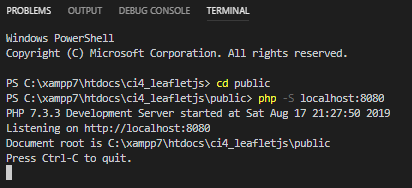
\includegraphics[width=0.5\textwidth]{figures/CODEIGNITER4/CI8.PNG}
	\end{figure}
	
	\vspace{4cm}
	\item Jalankan aplikasi \verb|ci4_leafletjs| anda pada browser kesayangan anda, dengan cara mengetikkan "localhost:8080", maka akan muncul tampilan seperti berikut:
	\begin{figure}[!htbp]
		\centering
		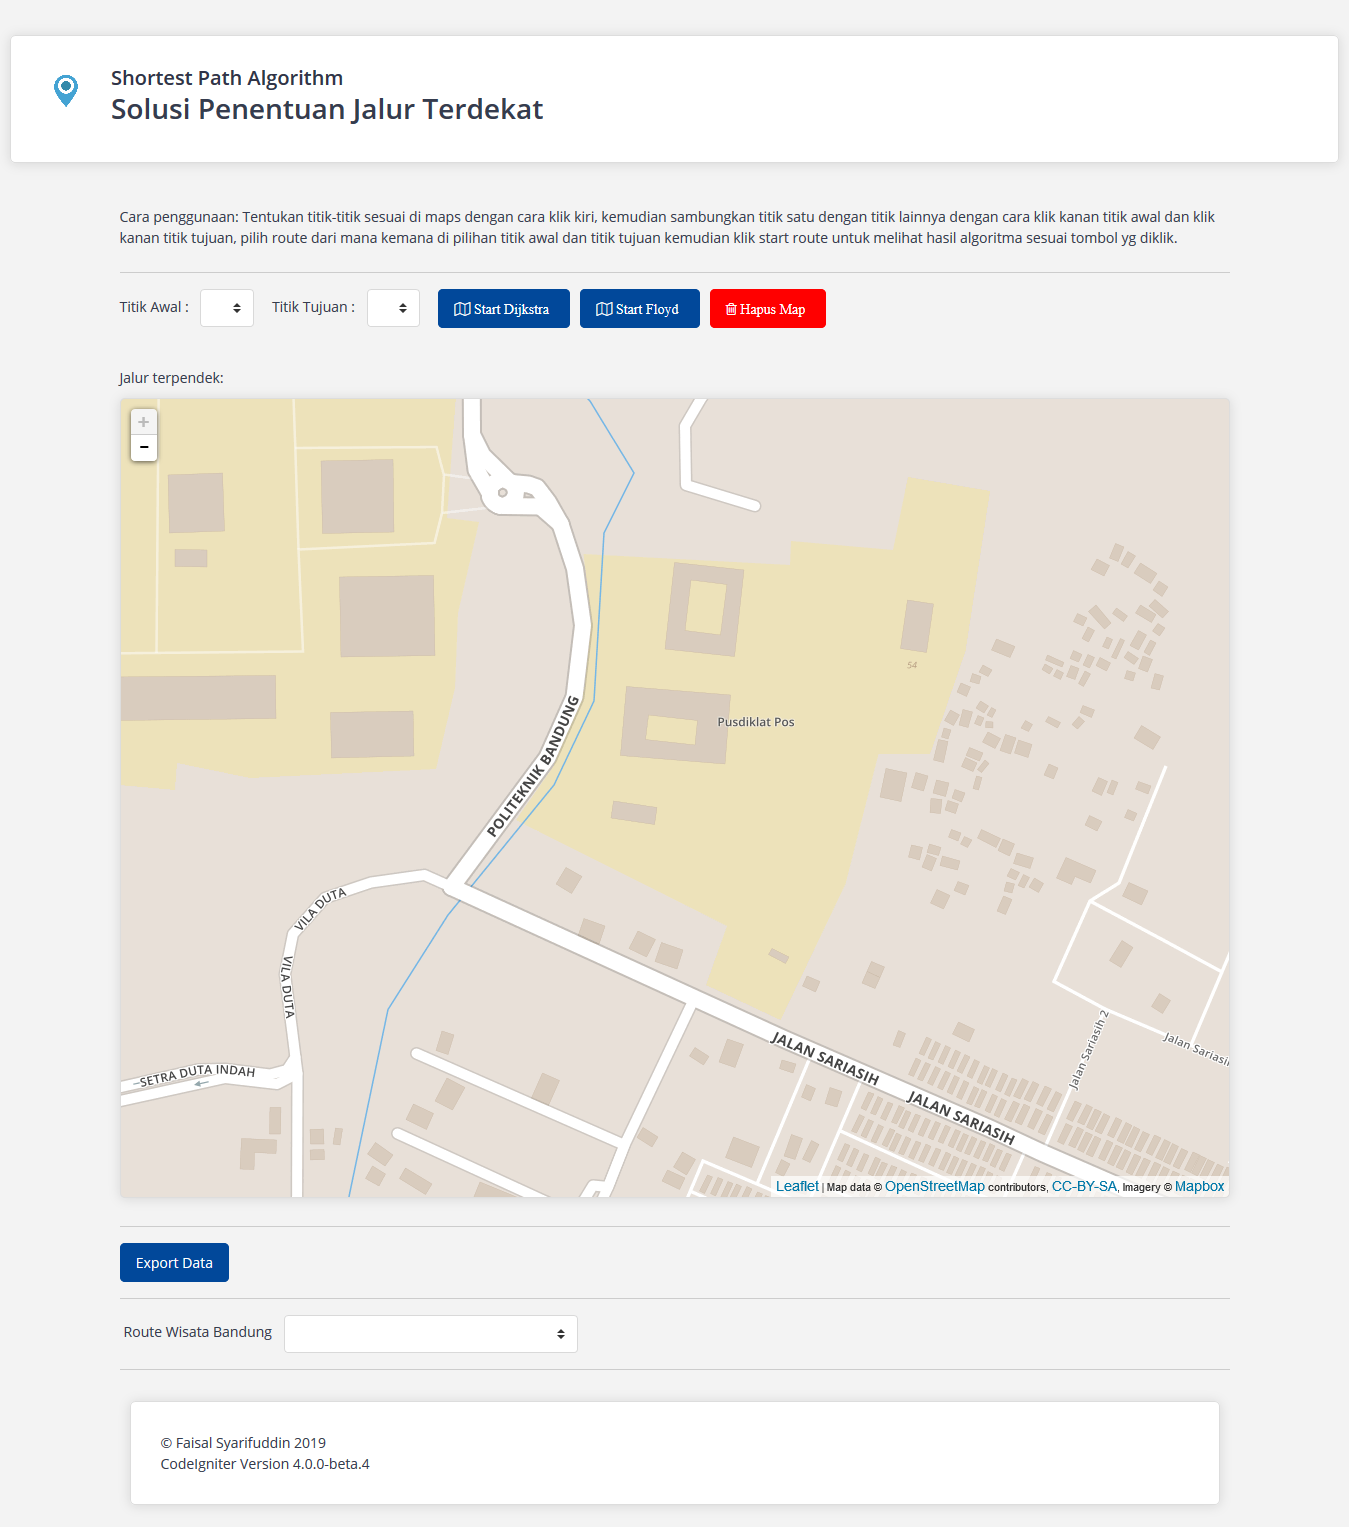
\includegraphics[width=0.5\textwidth]{figures/LEAFLETJS/LJS4.png}
		\label{Leaflet4}
	\end{figure}
	
\end{enumerate}

\bibliographystyle{IEEEtran} 
%\def\bibfont{\normalsize}
\bibliography{references}


%%%%%%%%%%%%%%%
%%  The default LaTeX Index
%%  Don't need to add any commands before \begin{document}
\printindex

%%%% Making an index
%% 
%% 1. Make index entries, don't leave any spaces so that they
%% will be sorted correctly.
%% 
%% \index{term}
%% \index{term!subterm}
%% \index{term!subterm!subsubterm}
%% 
%% 2. Run LaTeX several times to produce <filename>.idx
%% 
%% 3. On command line, type  makeindx <filename> which
%% will produce <filename>.ind 
%% 
%% 4. Type \printindex to make the index appear in your book.
%% 
%% 5. If you would like to edit <filename>.ind 
%% you may do so. See docs.pdf for more information.
%% 
%%%%%%%%%%%%%%%%%%%%%%%%%%%%%%

%%%%%%%%%%%%%% Making Multiple Indices %%%%%%%%%%%%%%%%
%% 1. 
%% \usepackage{multind}
%% \makeindex{book}
%% \makeindex{authors}
%% \begin{document}
%% 
%% 2.
%% % add index terms to your book, ie,
%% \index{book}{A term to go to the topic index}
%% \index{authors}{Put this author in the author index}
%% 
%% \index{book}{Cows}
%% \index{book}{Cows!Jersey}
%% \index{book}{Cows!Jersey!Brown}
%% 
%% \index{author}{Douglas Adams}
%% \index{author}{Boethius}
%% \index{author}{Mark Twain}
%% 
%% 3. On command line type 
%% makeindex topic 
%% makeindex authors
%% 
%% 4.
%% this is a Wiley command to make the indices print:
%% \multiprintindex{book}{Topic index}
%% \multiprintindex{authors}{Author index}

\end{document}

